%&pdflatex
\documentclass[11pt]{article}
\usepackage{algorithmicx}
\usepackage[ruled]{algorithm}
\usepackage{algpseudocode}
\usepackage{algpascal}
\usepackage{algc}
\usepackage{url,enumerate, amssymb, amsfonts}
\usepackage[colorlinks = true,
linkcolor = blue,
urlcolor  = blue,
citecolor = green,
anchorcolor = blue]{hyperref}
%\usepackage{setspace,listings}
\usepackage{graphicx}
\usepackage{amsmath}
\usepackage{psfrag}
\usepackage[font=small,labelfont=bf]{caption}
\usepackage{enumerate}
\usepackage{authblk}
\usepackage[sort&compress,comma,square,numbers]{natbib}
\usepackage{url} % not cruci
%\pdfminorversion=4
\usepackage{setspace}
\usepackage{lscape}
\usepackage{color,amssymb}
\usepackage{mathtools}
\usepackage{dcolumn}
\usepackage{indentfirst, verbatim, float}
\usepackage[margin=1.0in]{geometry}
%\newcounter{equationset, sectsty, breqn}
%\usepackage{setspace, amsmath,color}
%\usepackage{color,amssymb}
\usepackage{mathtools, amsthm, subcaption}
\theoremstyle{definition}
\newtheorem{definition}{Definition}[section]
\newtheorem{theorem}{Theorem}[section]
\newtheorem{corollary}{Corollary}[theorem]
\newtheorem{lemma}[theorem]{Lemma}
\newtheorem{remark}{Remark}
\bibliographystyle{unsrt}
\usepackage{sidecap}
\usepackage{titlesec}
\sidecaptionvpos{figure}{c}

% NOTE: To produce unblinded version, replace "0" with "1" below.
\newcommand{\blind}{0}
% DON'T change margins - should be 1 inch all around.
\newcommand{\cs}[1]{\textcolor{blue}{cs: #1}}

\begin{document}

\def\spacingset#1{\renewcommand{\baselinestretch}%
{#1}\small\normalsize} \spacingset{1}

%%%%%%%%%%%%%%%%%%%%%%%%%%%%%%%%%%%%%%%%%%%%%%%%%%%%%%%%%%%%%%%%%%%%%%%%%%%%%%
\title{\bf Nonparametric Network Dependence Testing by Diffusion Maps}
\if1\blind
{\author[1]{Youjin Lee (ylee160@jhu.edu)} %\thanks{cshen6@jhu.edu}}
	\author[2]{Cencheng Shen} %\thanks{cshen6@jhu.edu}}
	\author[2,3,4]{Joshua T. Vogelstein}
	\affil[1]{Department of Biostatistics, Johns Hopkins University}
  \affil[2]{Center for Imaging Science, Johns Hopkins University}
  \affil[3]{Department of Biomedical Engineering and Institute for Computational Medicine, Johns Hopkins University}
  \affil[4]{Institute for Data-Intensive Engineering \& Science, Johns Hopkins University}
  \date{}
	\maketitle
} \fi

	\if0\blind
	{
		\bigskip
		\bigskip
		\bigskip
		\begin{center}
			{\LARGE\bf Nonparametric Network Dependence Testing by Diffusion Maps}
		\end{center}
		\medskip
	} \fi

\begin{abstract}
%The text of your abstract. 200 or fewer words.
Deciphering the association of network structures with their nodal attributes of interest is a core problem in network science. As the network topology is structured and often high-dimensional, many traditional nonparametric tests are no longer applicable and instead parametric approaches are dominant in network inferences. We propose a new procedure for testing the dependence between network topology and nodal attributes. To deal with the structured data of the network, we introduce a family of random vectors, called diffusion maps, which embed each node into the Euclidean space. The diffusion maps then provide network metrics on which we apply nonparametric distance-based correlation tests. We demonstrate that our testing method, local optimal distance-based correlation test combined with proper network metrics, not only yields consistent test statistics under common network models, but also significantly surpasses the testing power of existing benchmarks under various circumstances. In particular when the amount of dependency differs between the nodes, the statistic not only efficiently detects the dependency but also measures each node's contribution to testing dependence. 
\end{abstract}

\noindent%
{\it Keywords:} testing independence, exchangeable graph, diffusion distance, distance correlation, multiscale generalized correlation

\sloppy
\doublespacing

\section{Introduction}
\label{sec:intro}
	\vspace*{-0.2cm}
	% General Backgrounds
Propelled by increasing demand and supply of graph data from various disciplines, the ubiquitous influence of network inferences has motivated numerous recent advances and applications in statistics, physics, computer science, biology, social science, etc., which further poses many new challenges to data scientists. One of the most fundamental statistical questions is to determine and characterize the relationship among multiple modalities of a given data set, for which the first step is to test the existence of any dependency between the data sets. However, the lack of a principal notion of correlation in the graph domain has not only hindered the progress of nonparametric dependency testing methods, but also deterred a rich literature of statistical techniques in other inferences (e.g., regression, feature screening, two-sample test) from being directly applied to graphs.
 
\subsection{Data Structure of Graph with Nodal Attributes}
A graph, or equivalently a network, can be formally defined as collection of nodes and edges.
Mathematically, a graph $\mathbf{G}=(V,E)$ can be formally defined as collection of a set $V$ of nodes (or vertices) and a set $E$ of edges, which is often represented via an adjacency matrix $\mathbf{A} = \{A_{ij} : i,j= 1,..,n = |V| \}$, e.g.~for an unweighted and undirected network $A_{ij} = 1$ if node $i$ and node $j$ are connected by an edge, and zero otherwise. Let $\mathbf{X} = \{  \mathbf{x}_{i} \in \mathbb{R}^{q_{x}} : i = 1, \ldots, n \}$ be nodal attributes, a random variable or random vector associated with each node. Assume that we are given a $n \times n$ adjacency matrix $\mathbf{A}$ and nodal attributes $\mathbf{X}$ for each of $n$ nodes. Since $\mathbf{A}$ is a symmetric square matrix when $\mathbf{G}$ is undirected, it does not satisfy traditional data assumptions, e.g., each observation can be assumed independently and identically distributed, the sample size increases faster than the feature dimension, etc.. These are the notable obstacles in directly applying conventional statistical methods. Therefore, graph inferences have long relied on specifying a particular statistical model for graphs, such as the Erdos-Renyi model \cite{erdosrenyi1959,Gilbert1959}, stochastic block model~\cite{HollandEtAl1983, rohe2011spectral,SussmanEtAl2012,Lei2015} and its degree-corrected version \cite{karrer2011stochastic, ZhaoLevinaZhu2012}, the latent position model~\cite{TangSussmanPriebe2013,fosdick2015testing}, the random dot product model~\cite{YoungScheinerman2007, sussman2014consistent}, etc. 
\begin{figure}[ht]
	\centering
	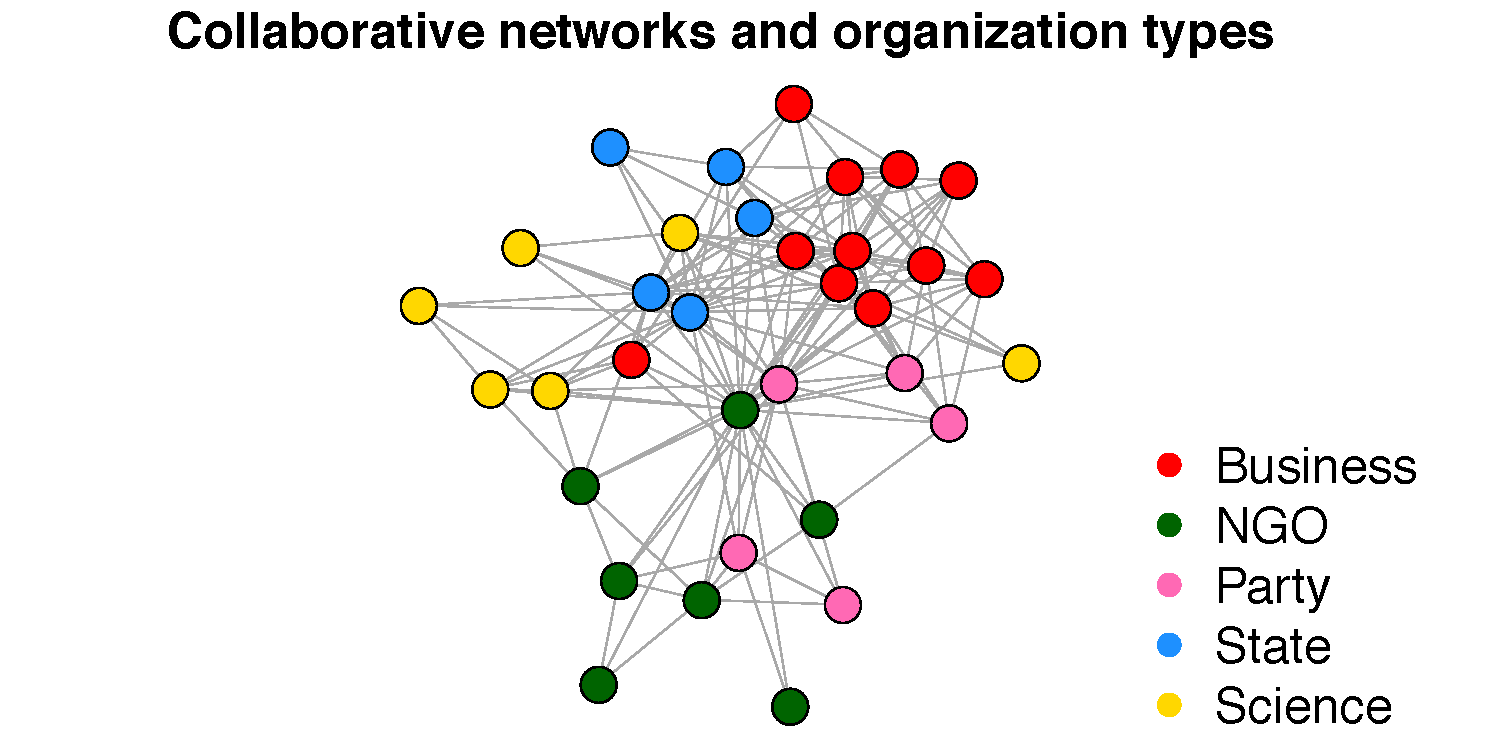
\includegraphics[width=4in]{introplot.pdf}	
	\caption{You may conjecture that organizations with the same type are more likely to collaborate each other at first glance; but there has been a lack of statistical method to test if there exists any significant relationship between network topology and node-specific attributes and if any, which node exerts the most dependency on network.}
	\label{fig:intro}
\end{figure}
However, model-based statistical methods often have limited applicability, e.g., connected-ness, unweighted-ness, and undirected-ness are the most common assumptions underlying statistical network models, which only represent a subset of real networks. Even under the model assumptions, how to select the model parameter can be expensive and unwarranted in practice, e.g., how to choose the dimension of latent factors for a given graph when a latent position model is assumed. Moreover, model mis-specification can largely affect the inference performance on networks. It is thus desirable to develop robust graph analysis approaches that are less dependent on models and parameters \cite{ChenShenVogelsteinPriebe2016}.

\subsection{Testing Network Dependence}
When it comes to investigating the relationships among network data, one of the core problems is to detect dependency between network topology and nodal attributes, i.e., certain properties of interest defined on the nodes. For example, each person on Facebook not only has a number of distinct attributes (e.g., occupations, sex, personal behaviors), but also interacts with other persons via the social network; in neuro-science, each brain region has its own distinct functionality, and is also connected with other regions in the brain map. Figure~\ref{fig:intro}, as an example, illustrates the collaborative networks between the political organizations which have different properties. Identifying dependency between network and nodal attributes, e.g. between collaborative relationships and the properties of each organization, however, has primarily focused on their relationship explained only by network model under the boundary of model assumption \cite{wasserman1996logit, fosdick2015testing, howard2016understanding}, thus suffers from the same problems all other model-based methods face. For example, the parametric network test proposed by Fosdick and Hoff \cite{fosdick2015testing} assumes a multivariate normal distribution of the latent factors as the generative model, estimates the latent factor of each node (which requires estimating its dimension $q$), then proceeds to test network dependence on the covariance by the standard likelihood ratio test. To our best knowledge so far, there is no principled method to compute a correlation measure on graphs which is consistent and model-free while overcoming all existing restraints on network analysis. 

\subsection{Testing Dependence in General Settings}
On the other hand, the general problem of dependence testing between two random vectors has seen notable progress in recent years. The Pearson's correlation~\cite{Pearson1895} is the most classical approach, which determines the existence of linear relationship via a correlation coefficient in the range of $[-1,1]$, with $0$ indicating no linear association while $\pm 1$ indicating perfect linear association. To capture all types of dependencies not limited to linear relationship, new correlation measures and nonparametric statistics have been suggested recently, such as the Mantel coefficient \cite{mantel1967}, RV coefficient \cite{RobertEscoufier1976}, distance correlation (\texttt{dCorr}) and energy statistic \cite{szekely2007measuring,szekelyRizzo2013a, RizzoSzekely2016}, kernel-based independence test \cite{GrettonGyorfi2010}, Heller-Heller-Gorfine (\texttt{HHG}) test \cite{HellerGorfine2013,heller2016consistent}, and multiscale generalized correlation (\texttt{MGC}) \cite{shen2016discovering}. In particular, the distance correlation by Szekely et al. \cite{szekely2007measuring} is the first correlation measure that is consistent against all possible dependencies (with finite moments). The multiscale generalized correlation statistic (\texttt{MGC}) by Shen et al. \cite{shen2016discovering} inherits the same consistency of distance correlation with remarkably better finite-sample testing powers under high-dimensional and nonlinear dependencies. The \texttt{MGC} defines a family of distance-based local correlations at every local scale and efficiently searches the optimal correlation in testing. Since all the above methods do not depend on particular models and also do not require explicit model parameter tuning, the network dependency testing may be significantly improved if some of them can be employed on graphs.

\subsection{Outline of the Article}
In the following Section~\ref{sec:method}, we introduce the background for network metrics and distance-based tests, which will be the ingredients for network dependence test. In Section~\ref{sec:theory} we demonstrate that our proposed test is theoretically sound under very mild condition, which includes almost all existing generative graph models while overcoming the theoretical barricades by the distinct structure of network data and relaxing the limitations of model-based method for network testing. Moreover, You can find in Section~\ref{sec:simulation} that our proposed statistic offers major power improvement under various scenarios in finite-sample testing. The combined advantages of the network metrics and the testing method over the existing benchmarks are illustrated via comprehensive simulations under popular network models.

%%%%%%%%%%%%%%%%%%%%%%%%%%%%%%%%%%%%%%%%%%%%%%%%%%%%%
\section{Method}
\label{sec:method}
\subsection{Diffusion Maps and Diffusion Distances}
\label{ssec:method2}

In this section, we introduce the diffusion maps as a family of network geometries for a graph \cite{coifman2006diffusion}. Coifman and Lafon~\cite{coifman2006diffusion,lafon2006diffusion} proposed multiscale geometries of data called diffusion maps, which are constructed by iterating the transition matrix that determines the probability of moving forward from one node to the others during the random walk. The transition matrix here can be based on any reasonable kernels that represent the similarity between the node while satisfying the assumptions~\cite{coifman2006diffusion, coifman2005geometric}. We are going to define such transition matrix $\mathbf{P}$ via an adjacency matrix as a kernel function. For example, given an undirected non-empty graph $\mathbf{G}$, we have $P_{ij} = A_{ij} / \sum\limits_{j=1}^{n} A_{ij}$ if $\sum\limits_{j=1}^{n} A_{ij} > 0$ and $P_{ij} = 0$ otherwise ($i,j=1,\ldots,n$). When this kernel satisfies the properties of symmetry, positivity, and positive semi-definiteness, all of which the transition matrix $\mathbf{P}$ based on a symmetric adjacency matrix obeys, the diffusion map $\mathbf{u}(i)$ corresponding to node $i$ at random walk iteration $t$ is computed as follows : 
\begin{align}
\label{eq:U}
\mathbf{u}_{t}(i)  &= \begin{pmatrix} \lambda^{t}_{1} \mathbf{\phi}_{1}(i) & \lambda^{t}_{2} \mathbf{\phi}_{2} (i)  & \cdots & \lambda^{t}_{q} \mathbf{\phi}_{q}(i) \end{pmatrix} \in \mathbb{R}^{q}; \quad i = 1, \ldots, n.
\end{align}
where $\{ \lambda_{j} \}$ and $\{ \phi_{j}  \}$ are the non-zero eigenvalues and corresponding eigenvectors of the transition matrix $\mathbf{P}$; $q$ is the number of non-zero eigenvalues; $\lambda^{t}_{j}$ is the $t^{\mbox{th}}$~power of the eigenvalue; and $(\cdot)^{T}$ is the matrix transpose. Then diffusion maps locate each node's position at every diffusion time $t$ and provide node-wise multivariate coordinates through $\{\mathbf{u}_{t}(i) : i = 1, \ldots, n;  t  \in \mathbb{N} \}$. It is not necessary to utilize whole set of non-zero eigenvalues in constructing diffusion maps but it is common to use a part of them having the largest absolute values considering the efficiency in dimensional reduction~\cite{coifman2006diffusion}. However since we are going to borrow the properties of transition matrix $\mathbf{P}$ to show that diffusion maps are independent sample under some conditions, deriving diffusion maps with a full set of $\{ \lambda_{j} \}$ and $\{ \phi_{j}  \}$ is required. A family of diffusion maps as a function of the eigenvalues and eigenvectors of $\mathbf{P}$ can always be obtained when a symmetric kernel is given. When a given non-empty graph $\mathbf{G}$ is directed, i.e. when the probability for a random walk from node $x (\in V)$ to $y (\in V)$ differs from that from $y$ to $x$, we are not able to represent diffusion maps via spectral properties of $\mathbf{P}$ based on an asymmetric kernel~\cite{tang2010graph} (Appendix~\ref{ssec:directed}). In that case we might set a new symmetric weight between node $i$ and node $j$, for example, $\tilde{w}_{ij}$, proportional to the average of both weights assigned to each direction, e.g. $\tilde{w}_{ij} := (w_{ij} + w_{ji} ) / 2$. From now on we are going to restrict our arguments to an undirected and unweighted graph for simplicity.

The \textit{diffusion distance} between node $i$ and node $j$, $C_{t}(i,j)$, considering the propagation of information through Markov chains at diffusion time $t$, is formally defined as follows:
\begin{equation}
\label{eq:distance}
C^2_{t}(i,j) := \sum\limits_{u \in V} \left( P^{t}_{iu} - P^{t}_{ju}  \right)^2 /  \pi(u),
\end{equation}
where $\pi(u)$ is a stationary probability of node $u (\in V)$. 
It has shown that the above diffusion distance is exactly equivalent to the Euclidean distance of the diffusion maps. 
\begin{equation}
\label{eq:diffusion}
C^2_{t}(i,j)  =   \parallel \mathbf{u}_{t}(i) - \mathbf{u}_{t}(j) \parallel   \quad i,j = 1,2, \ldots , n.
\end{equation}
As the diffusion time $t$ increases, the corresponding diffusion distance $C_{t}$ reveals the geometric structure of the network topology in a larger and larger scale, and is thus more likely to take into account of two nodes which are relatively difficult to reach each other when differentiating the distances of each pair. Figure~\ref{fig:diffusions} shows how well diffusion distance notices the community structure in a graph (generated by the stochastic block model by Equation~\ref{eq:Three}) while differentiating distances across blocks, when a reasonable $t$ is chosen in the family of diffusion distances $\{ C_{t} : t \in \mathbb{N} \}$. Compared to adjacent relation or geodesic distance, where the set of distances are differentiated as little as possible or as much as possible respectively, diffusion distance better reflects the connectivity since it considers every possible path between the two nodes in its computation. 

\begin{figure}[ht]
	\centering
	\begin{subfigure}[b]{0.23\textwidth}
		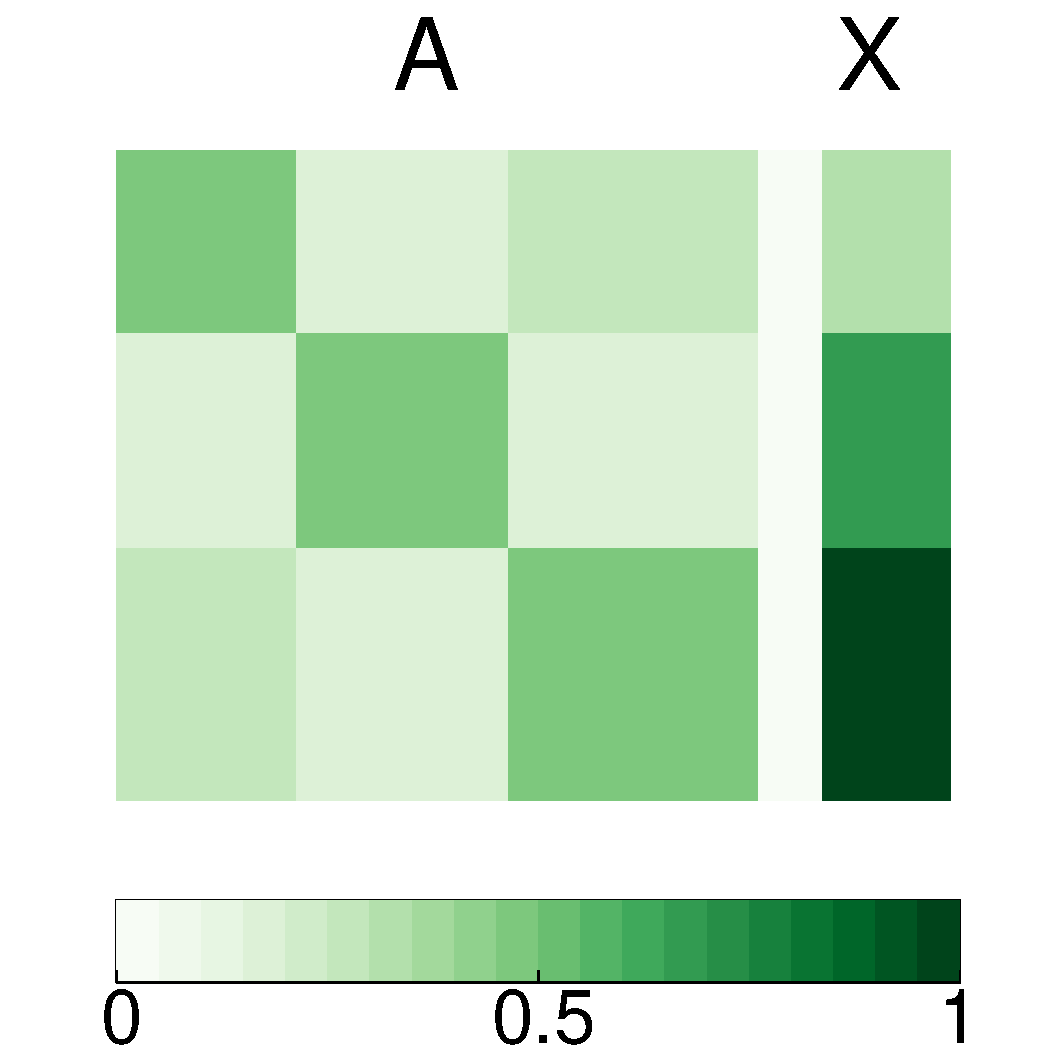
\includegraphics[width=\textwidth]{Pmat.pdf}
		\caption{}
		\label{fig:a}
	\end{subfigure}
	~ %add desired spacing between images, e. g. ~, \quad, \qquad, \hfill etc. 
	%(or a blank line to force the subfigure onto a new line)
	\begin{subfigure}[b]{0.23\textwidth}
		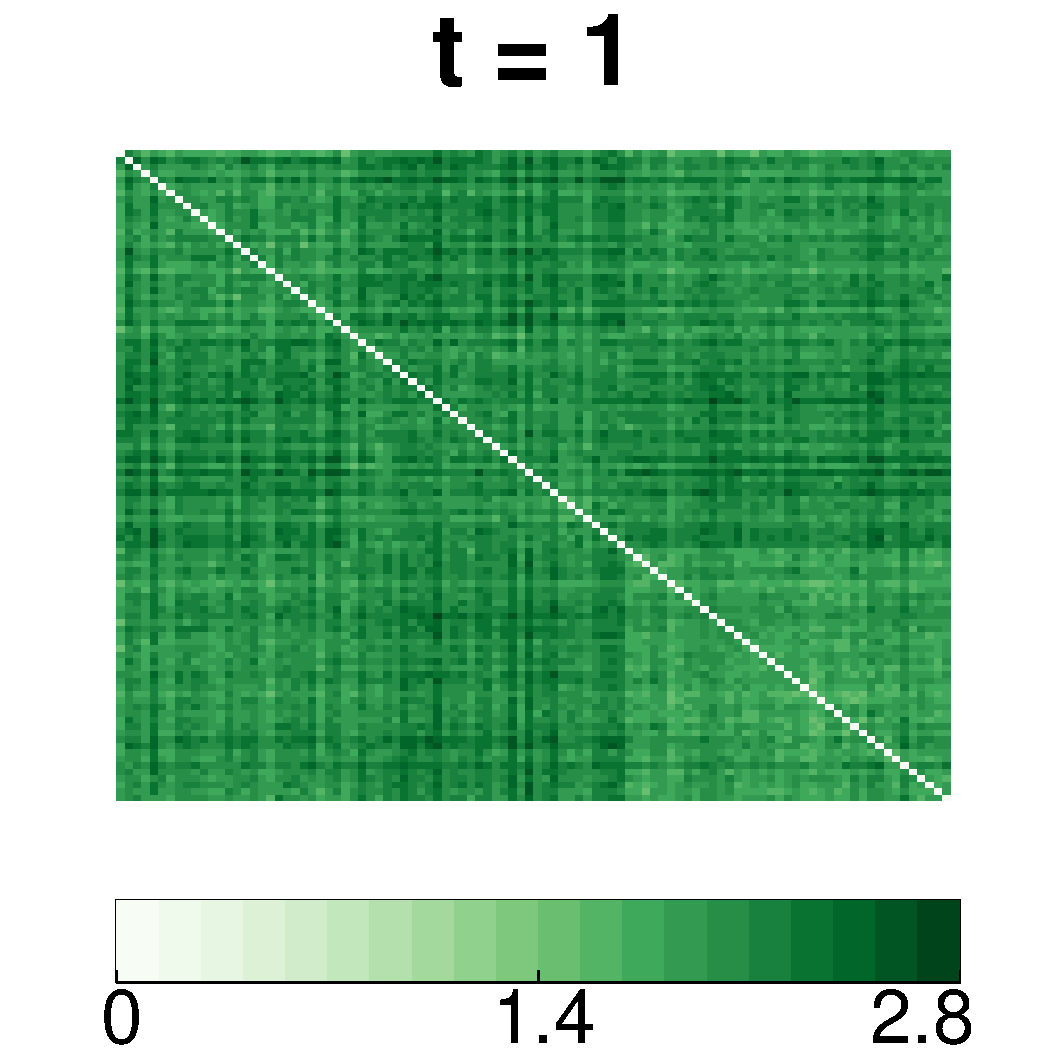
\includegraphics[width=\textwidth]{Dx1.pdf}
		\caption{}
		\label{fig:b}
	\end{subfigure}
	~ %add desired spacing between images, e. g. ~, \quad, \qquad, \hfill etc. 
	%(or a blank line to force the subfigure onto a new line)
	\begin{subfigure}[b]{0.23\textwidth}
		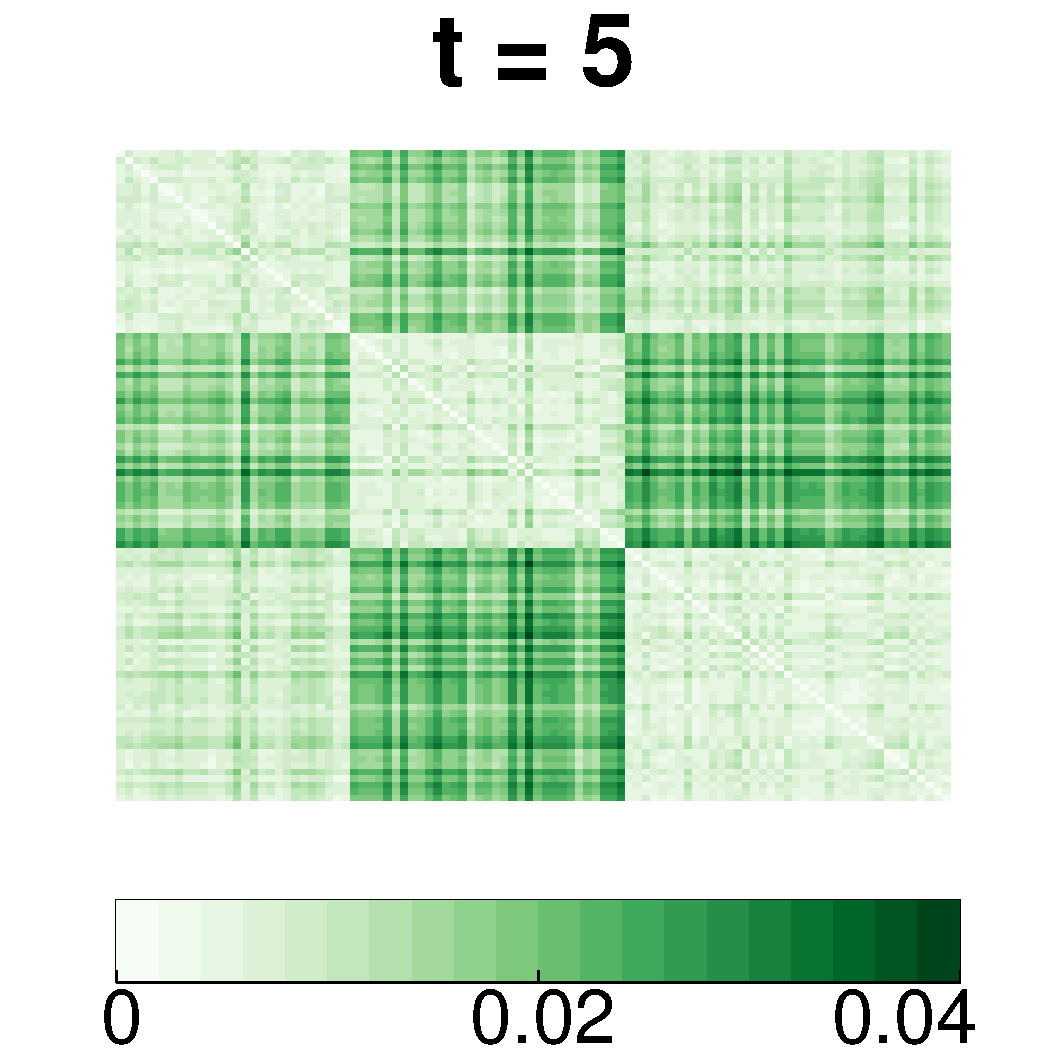
\includegraphics[width=\textwidth]{Dx5.pdf}
		\caption{}
		\label{fig:c}
	\end{subfigure}
	\begin{subfigure}[b]{0.23\textwidth}
		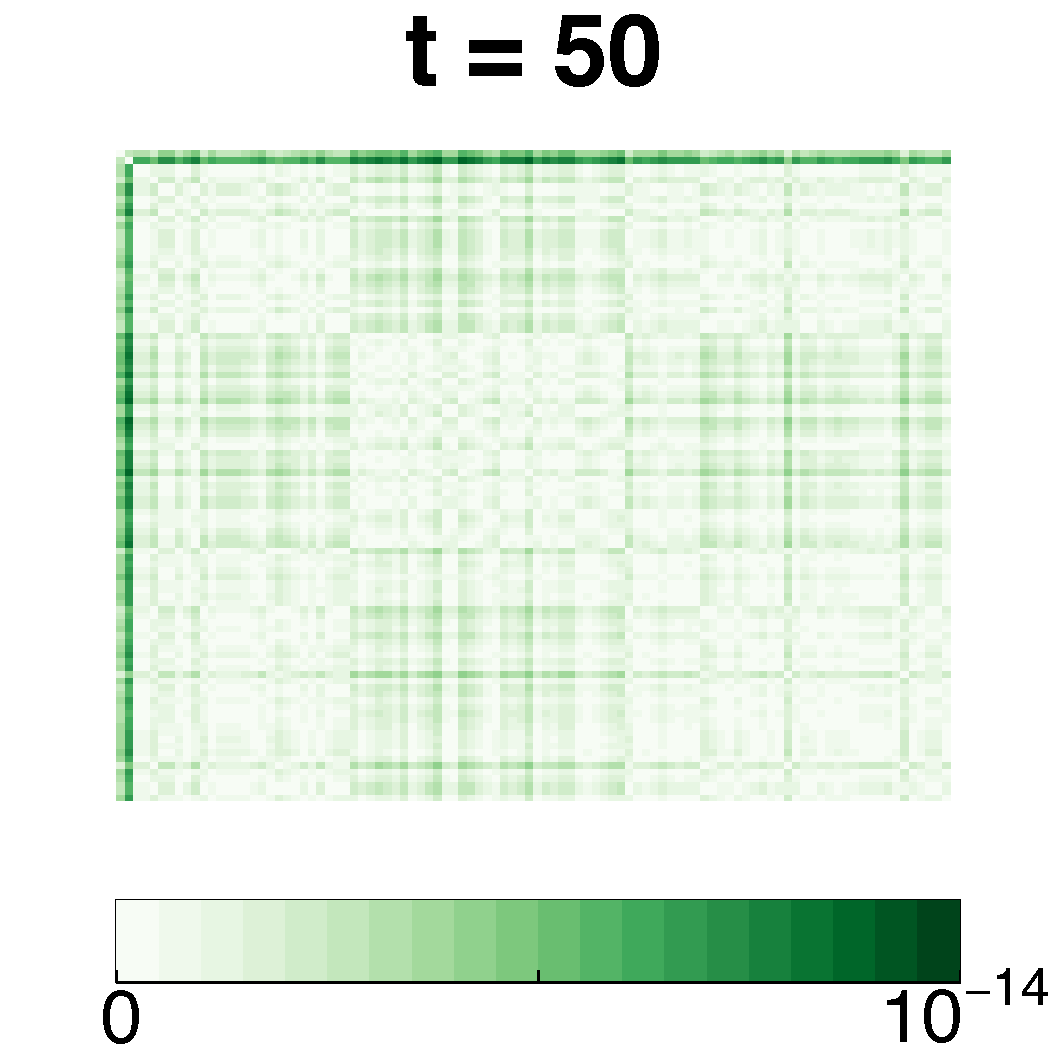
\includegraphics[width=\textwidth]{Dx50.pdf}
		\caption{}
		\label{fig:d}
	\end{subfigure}
	\caption{Panel (a) shows the adjacency matrix $\mathbf{A}$ and nodal attributes $\mathbf{X}$ generated by Equation~\ref{eq:Three}. Panel (b), (c), and (d) shows the diffusion distances of the graph, as a proposed network metric to provide a one-parameter family of network-based distances. As $t$ increases, there is a slight change in pattern, and the diffusion distance at $t = 5$ illustrates a very distinct block structures and thus has a very clear dependency to the attributes $\mathbf{X}$.}
	\label{fig:diffusions}
\end{figure}
\vspace*{-0.4cm}
Although the parameter $t$ may seem like another model parameter to tune, in practice $t \in [3,10]$ usually yields similar inference results. Therefore, throughout the paper we always take $t=5$ in the simulations, and drop the subscript $t$ in the diffusion maps $\mathbf{U}$ from now on. 

%%%%%%%%%%%%%%%%%%%%%%%%%%%%%%%%%%%%%%%
\subsection{Dependence Testing via \texttt{MGC}}
\label{ssec:method1}

The results in Section~\ref{ssec:method2} allow us to cast the network dependency test into the following framework: given sample data $(\mathbf{U}, \mathbf{X}) = \{  (\mathbf{u}_{i}, \mathbf{x}_{i} ) ; i = 1,2, \ldots, n \}$ defined as Equation~\ref{eq:U} that are identically distributed as $(\mathbf{u},\mathbf{x}) \in \mathbb{R}^{q \times q_x}$ ($q$ and $q_x$ are the respective feature dimension), we are looking to test whether their joint distribution equals the product of the marginals, i.e.,
\begin{align*}
& H_{0}: f_{\mathbf{u}\mathbf{x}}=f_{\mathbf{u}}f_{\mathbf{x}},\\
& H_{A}: f_{\mathbf{u}\mathbf{x}}\neq f_{\mathbf{u}}f_{\mathbf{x}}.
\end{align*}
If a pair of data $(\mathbf{u}_{i}, \mathbf{x}_{i} )$ can be further assumed independently distributed for each $i$, we can directly use a wide range of consistent test statistics, including the distance correlation, the \texttt{HHG} test, and \texttt{MGC}. Take the distance correlation for example: denote $C_{ij} = \parallel \mathbf{u}_{i} - \mathbf{u}_{j} \parallel$ and $D_{ij} = \parallel \mathbf{x}_{i} - \mathbf{x}_{j} \parallel$ for $i,j=1,2, \ldots ,n$, where $\parallel \cdot \parallel$ is the Euclidean distance. The sample distance covariance is defined as 
\begin{equation}	 
\label{eq:dCov}
\texttt{dCov}(\mathbf{U}, \mathbf{X}) = \frac{1}{n^2} \sum\limits_{i,j=1}^{n} \tilde{C}_{ij} \tilde{D}_{ij},
\end{equation}
where $\tilde{C}$ and $\tilde{D}$ is doubly-centered $C$ and $D$ by its column mean and row mean respectively, i.e., $\tilde{C}=HCH$, where $H=I_{n}-\frac{J_{n}}{n}$ (the double centering matrix), $I_n$ is the $n \times n$ identity matrix (ones on the diagonal, zeros elsewhere), and $J_n$ is the $n \times n$ matrix of all ones. The distance correlation (\texttt{dCorr}) follows by normalizing the distance covariance and is in the range of $[0,1]$. The best property of distance correlation is its consistency against almost all alternatives, i.e., $\texttt{dCorr}(\mathbf{U}, \mathbf{X})$ has testing power $1$ for sufficiently large $n$, for any joint distributions of finite second moment. In addition, a modified distance correlation (\texttt{mCorr}) was also proposed by Szekely and Rizzo~\cite{szekely2013distance} especially for testing high dimensional random vectors but unfortunately, the \texttt{mCorr} often fails to capture nonlinear associations especially embedded in high-dimensional data set~\citep{shen2016discovering, heller2012consistent}. 

The \texttt{MGC} test inherits the consistency of distance correlation and significantly improves the finite-sample testing power via utilizing the correlation from a subset of data points. To be specific, we first compute all local covariances $c^{kl}_{n}$ still based on the distance matrices of $\mathbf{U}$ and $\mathbf{X}$ but only including up to $k$-nearest points and up to $l$-nearest points for each data set. 
% include the MGC statistic
\begin{equation}
\label{eq:MGC}
c^{kl}_{n} = \frac{1}{n^2} \sum\limits_{i,j=1}^{n} \tilde{C}_{ij} \tilde{D}_{ij} I\big( r(C_{ij}) \leq k \big) I\big(  r(D_{ij}) \leq l  \big), \quad k= 1, \ldots, K_{\mathbf{U}}; l =1, \ldots, L_{\mathbf{L}},
\end{equation}
where %$C^{k}_{ij} = C_{ij} - \bar{C}^{k}$ and $D^{k}_{ij} = D_{ij} - \bar{D}^{k}$ with local mean $\bar{C}^{k}$ and $\bar{D}^{l}$; 
$r(C_{ij})$ denotes a rank function of data $\mathbf{U}$ indicating the rank of $\mathbf{u}_{i}$ with respect to $\mathbf{u}_{j}$, and the same definition for $r(D_{ij})$ in data $\mathbf{X}$; 
%$\sigma^{k}_{C}$ and $\sigma^{l}_{D}$ denote the standard deviations for the truncated pairwise comparison in data $\mathbf{U}$ and data $\mathbf{X}$ respectively; 
$K_{\mathbf{U}} (\leq n)$ and $L_{\mathbf{X}} (\leq n)$ is the number of distinct values in data $\mathbf{U}$ and $\mathbf{X}$ respectively. Then the local correlations are the normalizations of the local covariance into $[-1,1]$, and the MGC statistic is denoted by $c^{k^{*} l^{*}}_{n}$ via locating the optimal choice of neighborhood $(k^{*}, l^{*})$ among all possible neighborhood choices.
\cs{I rephrased the above MGC definition a little. Still need a few tweaks later. Better explain a bit on computation advantage, and what it means to be optimal here. }


%%%%%%%%%%%%%%%%%%%%%%%%%%%%%%%%%%%%%%%%%%%%%%%%%
\section{Theoretical Properties}
\label{sec:theory}

However, as the \textit{i.i.d.} assumption on $\mathbf{U}$ is not satisfied under network topology, the consistency of distance correlation is no longer guaranteed when applied to the arbitrary distance metric of the graph. In particular, neither the Euclidean distance of the adjacency vector nor the shortest-path distance can work together with distance correlation without breaking its consistency proof. We are going to introduce one of the statistical network models under which diffusion maps provide \textit{i.i.d.} network observations. 

A graph $\mathbf{G}$ is called exchangeable if and only if its adjacency matrix $\mathbf{A}$ is jointly exchangeable \cite{orbanz2015bayesian}, i.e.~for every permutation $\sigma$ of $n$ elements, $(A_{ij}) \stackrel{d}{=} (A_{\sigma(i) \sigma(j)})$. Exchangeability is a mild condition that most generative statistical network models satisfy, including all aforementioned models such as the stochastic block model and latent position model \cite{rohe2011spectral, sussman2014consistent, todeschini2016exchangeable}. Lemma~\ref{main_lemma} proves that the diffusion map as node-wise multivariate coordinates $ \mathbf{U}_{t} =  \{ (\mathbf{u}_{t}(1), \mathbf{u}_{t}(2), \cdots, \mathbf{u}_{t}(n)   )    : t \in \mathbb{N} \}$ can furnish conditional \textit{i.i.d.} samples for nodes in an exchangeable graph, with the proof supplied in the Appendix.
\begin{lemma}[Conditional \textit{i.i.d.} of diffusion map $\mathbf{U}_{t}$]
	\label{main_lemma}
	Assume that $\mathbf{G}$ is an exchangeable random graph. Then as $n \rightarrow \infty$, the diffusion map $\{ \mathbf{u}_{t}(i) : i = 1, \ldots, n \}$ are conditionally \textit{i.i.d.} given its underlying distribution.  
\end{lemma}

Now assume that $\mathbf{G}$ is an exchangeable random graph and its diffusion maps are $\mathbf{U}$ with finite moment; and the nodal attributes $\mathbf{X}=\{ \mathbf{x}_{i}: i = 1,2, \ldots, n \}$ are \textit{i.i.d.} as a random vector $\mathbf{x}$ of finite moment. Lemma~\ref{main_lemma} shows that $\{ \mathbf{u}_{i} : i = 1, \ldots, n  \}$ are conditional \textit{i.i.d.} for an exchangeable graph, i.e., there exists an underlying distribution random variable $\mathbf{u}$ such that $\mathbf{u}_{i}|\mathbf{u}$ are \textit{i.i.d.} as $n \rightarrow \infty$. The following two Lemmas serve as the foundation for using exchangeable observations in distance-based independence testing. 

\begin{lemma}
	\label{lemma1}
	Let $\mathcal{V}^2_{n}(\mathbf{U}, \mathbf{X})$ be the distance covariance (\texttt{dCov}) of $(\mathbf{U}, \mathbf{X}) = \{  ( \mathbf{u}_{i}, \mathbf{x}_{i}  )  : i = 1, \ldots, n \}$ defined as Equation~\ref{eq:dCov}.
	Then we have 
\begin{eqnarray}
		\mathcal{V}^{2}_{n}(\mathbf{U},\mathbf{X}) &=   \|g_{\mathbf{u},\mathbf{x}}^{n}(t,s)-g_{\mathbf{u}}^{n}(t)g_{\mathbf{x}}^{n}(s)\|^{2},
\end{eqnarray}
	where $g_{\cdot}^{n}$ is the \textit{empirical} characteristic function based upon $\{(\mathbf{u}_{i},\mathbf{x}_{i}) : i=1,2,...,n\}$
\end{lemma}

\begin{lemma}
	\label{lemma2}
	Then under the conditions above on $(\mathbf{U}, \mathbf{X})$, we have 
	\begin{eqnarray}
	\mathcal{V}_{n}^{2}(\mathbf{U},\mathbf{X}) &\longrightarrow \mathcal{V}^{2}(\mathbf{u},\mathbf{x}) \quad \quad \mbox{ as } n \rightarrow \infty
	\label{eq:conv1}
	\end{eqnarray}
	where $\mathcal{V}^{2} (\mathbf{u},\mathbf{x}) := \| g_{\mathbf{u},\mathbf{x}}(t,s) - g_{\mathbf{u}}(t) g_{\mathbf{x}}(s) \|^2$, and $g_{\cdot}$ is a characteristic function, e.g., $g_{\mathbf{u},\mathbf{x}}(t,s) = E\{\exp\{i \left\langle t,\mathbf{u} \right\rangle  +i \left\langle  s,\mathbf{x}\right\rangle \}\}$.
	It follows that 
	\begin{eqnarray}
	\mathcal{V}_{n}^{2}(\mathbf{U},\mathbf{X}) &\rightarrow 0 \quad \mbox{ as } n \rightarrow \infty
	\label{eq:conv2}
	\end{eqnarray}
if and only if $g_{\mathbf{u},\mathbf{x}}(t,s) = g_{\mathbf{u}}(t) g_{\mathbf{x}}(s)$, i.e., $\mathbf{u}$ is independent of $\mathbf{x}$.
\end{lemma}

Followed by Lemma~\ref{main_lemma}, Lemma~\ref{lemma1} and Lemma~\ref{lemma2}, our next result shows that both the \texttt{dCorr} and \texttt{MGC} defined on the diffusion distance can have the same consistency when extended to network dependency test of exchangeable graphs.

\begin{theorem}[\texttt{MGC} Consistency via Diffusion Distance]
Under the conditions above, 
$$\texttt{dCorr}(\mathbf{U}, \mathbf{X}) \longrightarrow 0 \mbox{ as } n \rightarrow \infty$$ 
if and only if $\mathbf{U}$ is independent of $\mathbf{X}$. And both \texttt{MGC} and \texttt{dCorr} are consistent for testing independence between any $\mathbf{U}$ and $\mathbf{X}$ satisfying the above condition.
	\label{theoremMain}
\end{theorem}

Therefore, our approach not only yields an easy-to-use methodology in network dependence testing, but also enjoys solid theoretical property and thus offers a principal approach to study correlation on network data. You can find the proof of this theorem in Appendix~\ref{ssec:proof}.

\cs{I think, maybe we should take certain contents out of Section 2, and make a separate review section on diffusion maps and MGC. Then in the results section, we can be more concentrated and clearer about our contribution and theorems. Also add another subsection describing the full network testing procedure. What do you think?}
\textcolor{red}{I am very certain what it does mean but I agree that we now have heavy section 2. Let us discuss this next week.}

\cs{For the directed case, if it does not work we simply exclude; otherwise we can either add it here or in the appendix (so as not to further complicate the main content)}
\textcolor{red}{As long as I found, spectral decomposition diffusion maps of asymmetric weight matrix is not tractable; so it is not unusual to transform asymmetric kernel to the symmetric. Why don't we just mention one sentence suggesting such alternatives?  }
%Note that if $\{ \mathbf{w}_{i} : i = 1,2,\ldots, n \}$ are \textit{i.i.d}, they are also exchangeable. Thus estimated latent network factors, which are assumed \textit{i.i.d} by \cite{fosdick2015testing} can also be applied to Theorem~\ref{theoremMain}. We already have shown that even under undirected network, diffusion maps remain exchangeable at each diffusion time point $t$. 

%%%%%%%%%%%%%%%%%%%%%%%%%%%%%%%%%%%%%%%%%%%%%%%%%
\subsection{Node Contribution to Testing Dependence}

On the other hand, in the presence of nonlinear dependency, some nodes often exert more reliance on their attributes than the others. Like other node-specific measures of importance, e.g. centrality,  the amount of each node's leverage on dependence can be of interest. Here we suggest the measure of node's contribution to detecting dependence by utilizing \texttt{MGC} statistic. Let $(k^{*}, l^{*})$ be the optimal neighborhood choice in the distance matrix $(C, D)$ respectively. Denote the contribution of node $v \in V(\mathbf{G})$ to the testing statistic by  $h(\cdot) : v \rightarrow \mathbb{R}$
\begin{equation}
\label{eq:contribution}
h(v) =  \frac{1}{n} \sum\limits_{j=1}^{n} C_{j v} D_{j v} I \big(  r (C_{j v}) \leq k^{*}  \big) I \big( r (D_{ j v }) \leq l^{*} \big), 
\end{equation}
which is proportional to $v^{th}$ column-sum of the pre-summed test statistic~\ref{eq:MGC} at optimal neighborhood choice. Note that the deviation of non-negative \texttt{MGC} statistic from zero implies departure from the independence and also note that we truncate the \texttt{dCov} statistics by column entry's rank. Thus $C_{jv} D_{jv}$ would not be truncated if node $j$ $(\in \{ 1,2, \ldots, n \} \setminus v )$ is important to node $v$ and its larger, positive value would contribute to $h(v)$ more. The statistic $c(v)$ comes out from these observations. 

\begin{theorem}[\textcolor{red}{Node contribution theorem}]
	\label{contributiontheorem}
	Assume two nodes $u$ and $v$ in a given network $\mathbf{G}$, i.e., $u, v \in V(\mathbf{G})$ and network topology associated with node $u$  is dependent on the attributes $X$ associated with node $u$; while network topology of $v$ is independent of the nodal attributes of $v$. Then $P\big(  h(u)  \geq h(v) \big) \longrightarrow 1$ as $n \rightarrow \infty$.
\end{theorem}	
\cs{I will rephrase this theorem.}
\textcolor{red}{I will think about contribution theorem after doing real data experiment enough.}


%%%%%%%%%%%%%%%%%%%%%%%%%%%%%%%%%%%%%%%%%%%%%%%%%%
\section{Simulation Study}
\label{sec:simulation}
	\vspace*{-0.2cm}
Next we investigate our approach via simulated models and empirical performances. In the simulation studies, we compare the empirical testing powers of four test statistics: \texttt{MGC}, \texttt{mCorr}, \texttt{HHG}, and the likelihood ratio test proposed by Fosdick and Hoff (\texttt{FH})~\cite{fosdick2015testing}. For the first three statistics, we further consider three different metrics of the network topology: the Euclidean distances of the diffusion maps (\texttt{DM}), of each column of adjacency matrix (\texttt{AM}), and of the latent factors (\texttt{LF}), which is based on singular value decomposition of the adjacency matrix. The \texttt{FH} likelihood ratio test must always be based on the latent factors.

Note that the latent-factor-based \texttt{FH} test requires a selection of a dimension parameter $q$, which we vary $q \in [1,10]$ and take the optimal power within the range (e.g., as a benchmark, the \texttt{FH} test actually has its power maximized over the parameter range). While for the diffusion maps, it suffices to fix $t=5$ as discussed in Section~\ref{ssec:method2}.

For each simulation model and each test, we repeatedly generate sample graph and attributes for $500$ times, carry out the permutation test, and reject the null if the resulting p-value is less than $\alpha = 0.05$. The testing power of each method equals the percentage of correct rejection. 

\subsection{Stochastic Block Model}

Let us first consider SBM with $3$ blocks, i.e., partition the nodes into $3$ communities, and generate the edges by a Bernoulli random variable whose probability is determined by the communities of the connecting nodes. Assume $n=100$ nodes whose attribute values $\mathbf{x}_i$ takes values of $0,1,2$ in ordinal scale equally likely. The edge probability is designed as
\begin{equation}
\label{eq:Three}
E(A_{ij} | X_{i}, X_{j}) = 0.5 I(|X_{i} - X_{j}| = 0) + 0.2 I(|X_{i} - X_{j}| = 1) + 0.3 I(|X_{i} - X_{j}| = 2), \quad i,j = 1, \ldots, n = 100.
\end{equation} 
Namely, within-block edge probability is $0.5$, between-block edge probability is $0.2$ or $0.3$ depending on the communities defined by (dis)similarity in nodal attributes value of $X$. This 3-block model describes a nonlinear dependency, where \texttt{MGC} has been shown to work better than the \texttt{dCorr} given a pair of random vectors~\cite{shen2016discovering}. We now want to look at the performance of \texttt{MGC} given a graph object and a random vector of nodal attributes. A visualization of the statistics from one sample graph is offered in Figure~\ref{fig:diffusions}. After repeatedly generating the data set and implementing independence testing by all the methods mentioned, the powers are computed and shown in Figure~\ref{fig:threeSBM}, for which \texttt{MGC} combined with diffusion maps indeed yields the most superior power comparing to all other benchmarks.

\begin{SCfigure}[][ht]
	\centering
	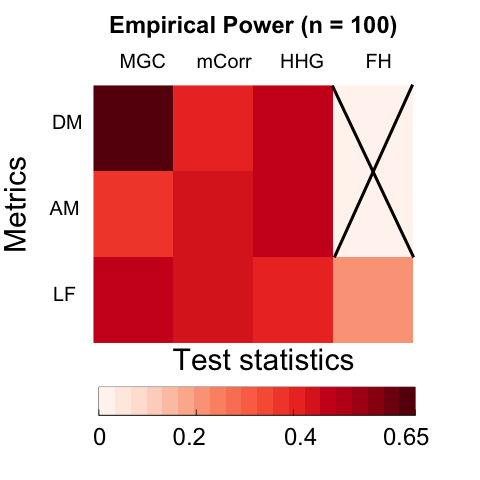
\includegraphics[width=0.4\paperwidth, height=0.4\paperwidth]{ThreeSBM.png}
	\caption{The power heatmap under the SBM with three blocks (Equation~\ref{eq:Three}) demonstrates that for all possible combinations of test statistics with distance metrics the \texttt{MGC} with the diffusion maps yields the best power comparing to all other methods.}
	\label{fig:threeSBM}
\end{SCfigure}

To further understand the advantage of \texttt{MGC}, we fix the diffusion distance as the network metric, and compare different test statistics. Based on the same three-block model, the edge probability is now generated as follows,by controlling the amount of \textit{nonlinear dependency} through $\theta \in (0, 1)$:
\begin{equation}
E(A_{ij} | X_{i}, X_{j}) = 0.5 I(|X_{i} - X_{j}| = 0) + 0.2 I(|X_{i} - X_{j}| = 1) + \theta I(|X_{i} - X_{j}| = 2), \quad i,j = 1, \ldots, n = 100.
\label{eq:mono}
\end{equation}
When $\theta > 0.2$, the network dependency changes from a close to linear relationship to strongly nonlinear. Figure~\ref{fig:powerplot} shows the testing power with respect to increasing $\theta$, and there is a clear trend that both the \texttt{dCorr} and \texttt{FH} tests have deteriorating power while \texttt{MGC} has a very stable performance against varying $\theta$. The same phenomenon holds by varying other edge probabilities. These observations support the argument that the \texttt{MGC} can better capture the nonlinear dependencies for network dependence testing, and is the best method to couple with the diffusion distance.
\begin{figure}[ht]
	\centering
	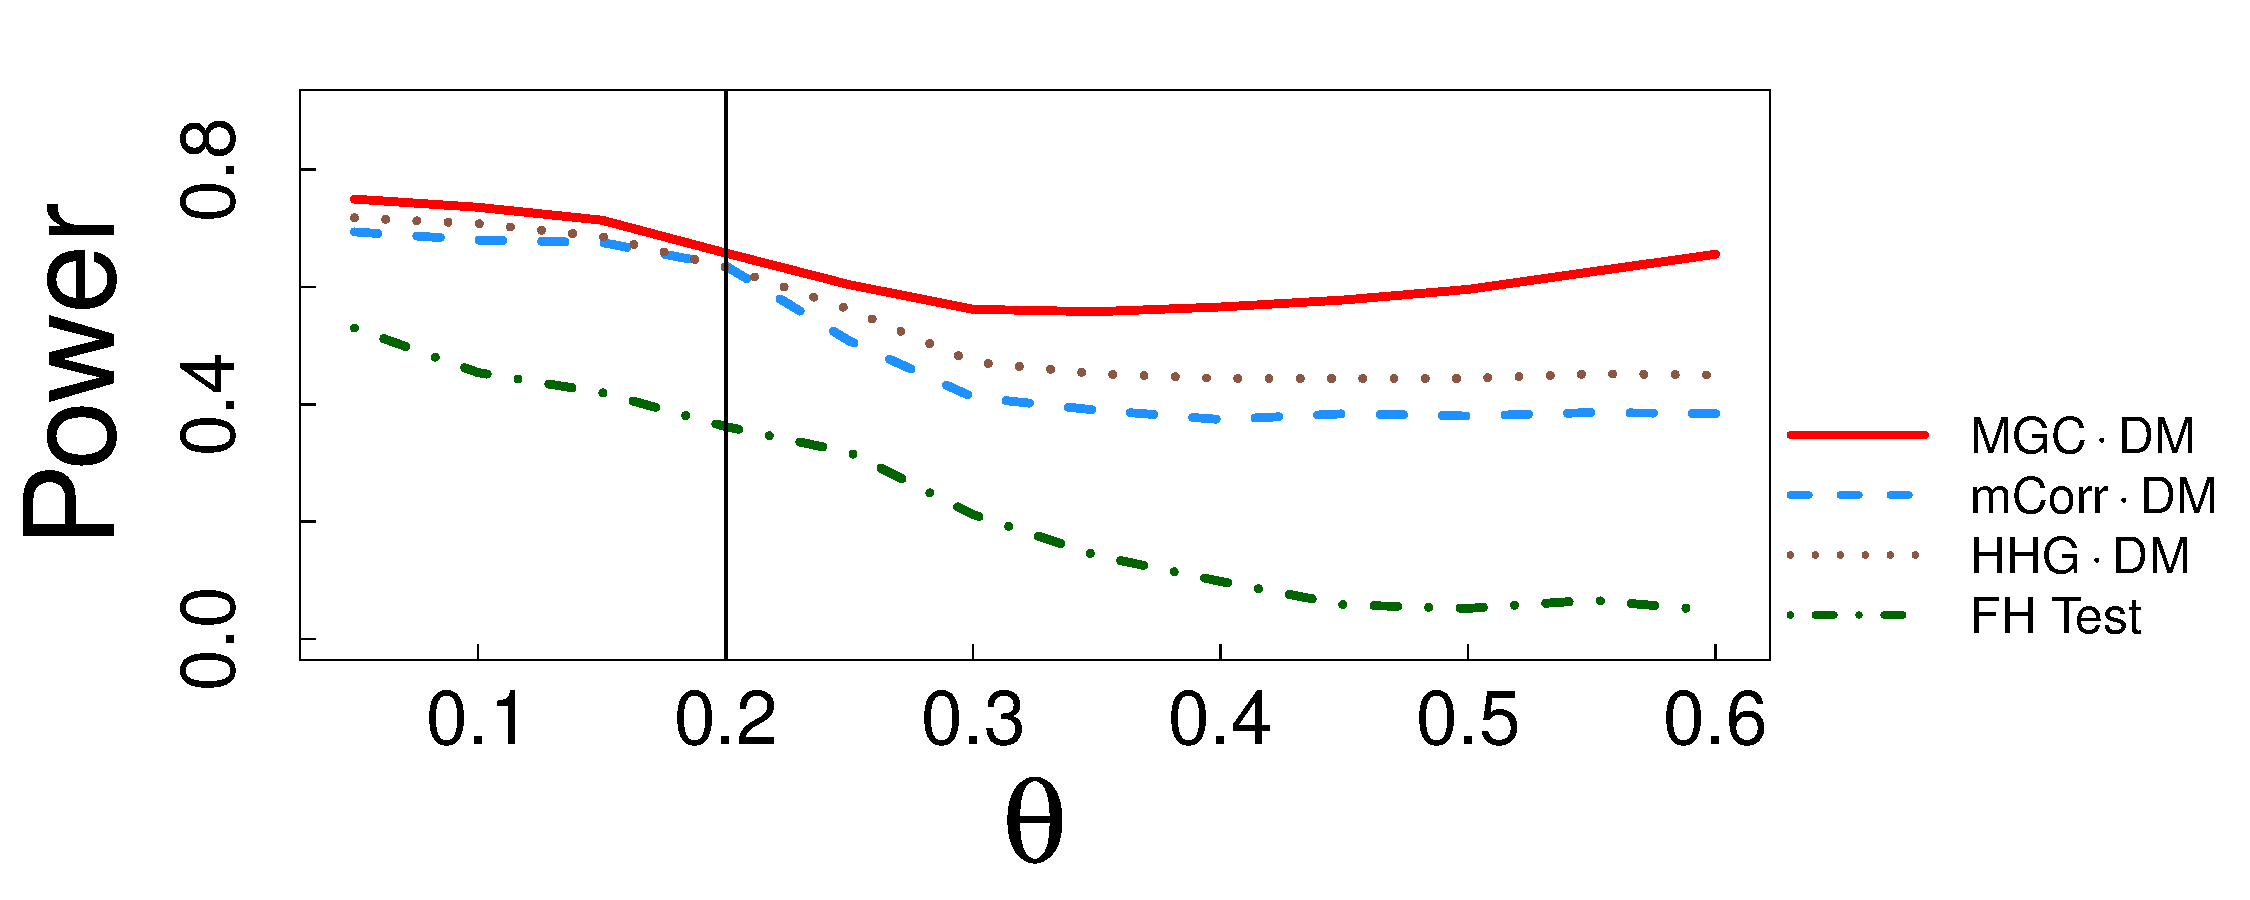
\includegraphics[width=0.7\linewidth]{mono.pdf}
	\caption{The power curve with respect to increasing $\theta$ in the SBM with three blocks, for \texttt{MGC}, \texttt{mCorr}, and \texttt{FH}. Larger $\theta$ implies stronger nonlinear dependency, while $\theta<0.2$ has close-to-linear dependency. The \texttt{MGC} is the best performing method throughout all possible $\theta$.} 
	\label{fig:powerplot}
\end{figure}

\subsection{Degree-corrected Stochastic Block Model}
% degree-corrected two block model
Our next simulation shifts to the degree-corrected stochastic block model (DC-SBM) with two blocks. The DC-SBM adds another random variable $V_{i}$ associated with each node to vary the node degrees, which is a generalization of the stochastic block model and provides a better fit to real networks. Setting $n=250$, suppose that the nodal attributes $X_i$ takes binary values in $0$ and $1$ equally likely, and the edge probabilities are specified by  
\vspace*{-0.4cm}
\begin{equation}
E( A_{ij} | \mathbf{X}, \mathbf{V} )  = 0.2 V_{i} V_{j} \cdot I ( |X_{i} - X_{j}| = 0 ) + 0.05 V_{i} V_{j} \cdot I(|X_{i} - X_{j}| = 1),
\label{eq:tau}
\vspace*{-0.4cm}
\end{equation} 
where $V_{i} \overset{i.i.d}{\sim} Uniform(1 - \tau, 1 + \tau)$ for $i = 1, \ldots, n$, and $\tau$ $(\in [0, 1])$ is a parameter to control the amount of variability in the edge distribution. Again, the \texttt{MGC} coupled with diffusion maps, i.e. $\texttt{MGC} \circ \texttt{DM}$, is the best method in power throughout $\tau$; and in Figure~\ref{fig:combined} (a) we show the testing power restricted to $\texttt{MGC}$ but varying the distance metrics, which shows the diffusion distance is indeed the best distance metric for network dependence testing.

\begin{figure}[ht]
	\centering
	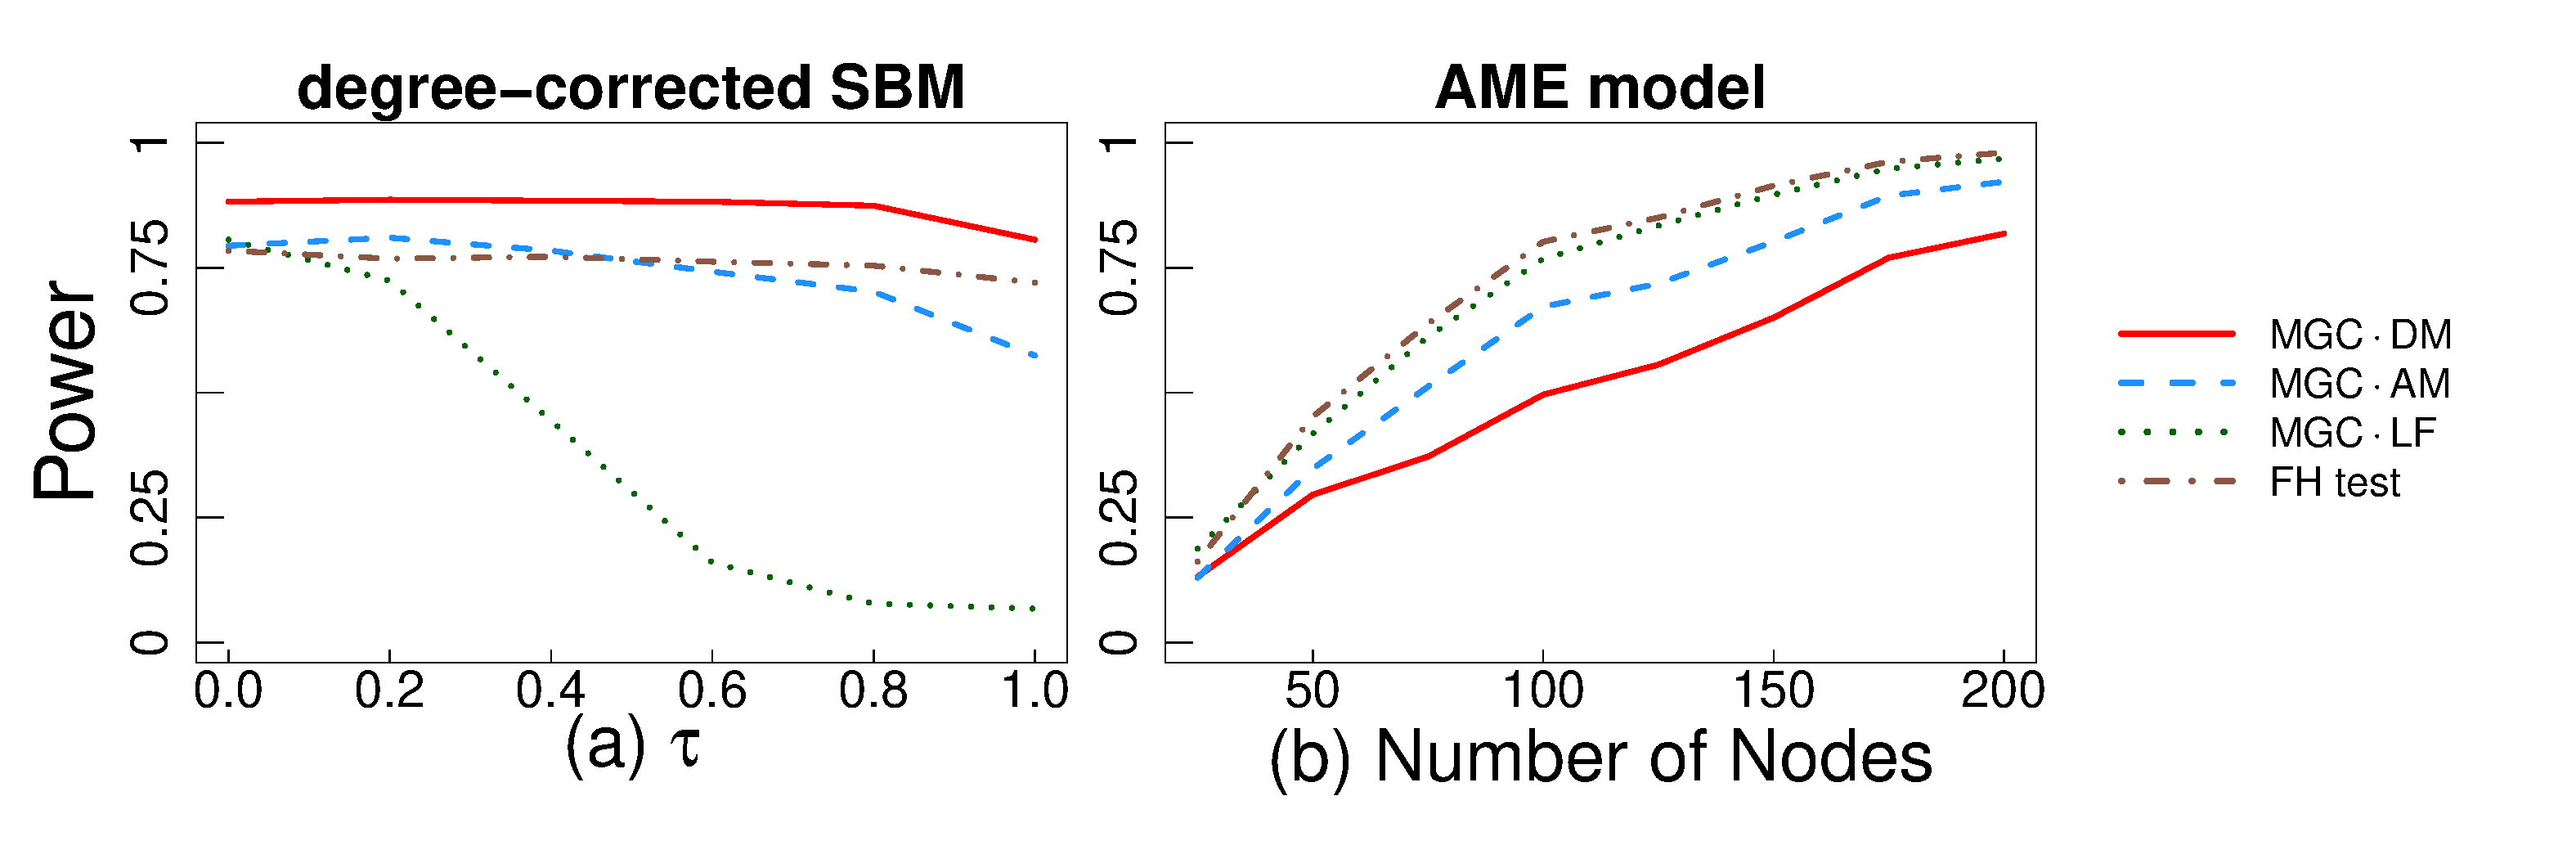
\includegraphics[width=\textwidth]{amedc.pdf}
	\caption{(a) In DC-SBM where the variability in degree distribution increases as $\tau$ increases, testing power of diffusion maps are more likely to be robust against increasing variability compared to other network metrics, e.g. adjacency matrix or latent positions. The \texttt{FH} test statistics allowing different dimensions of network factors perform consistently well but still have less power than the \texttt{MGC}. (b) The \texttt{MGC} utilizing diffusion distances loses some power under additive and multiplicative model which favors estimated latent position metrics, but \texttt{MGC} does as good as \texttt{FH} tests under latent factor metrics which closes to the truth. This reveals the flexibility in selecting distance matrix used in \texttt{MGC} statistics, which can be chosen depending on model fit or preliminary knowledge.}
	\label{fig:combined}
\end{figure}	

\subsection{Additive and Multiplicative Graph Model}
\label{ssec:ame}

Fosdick and Hoff~\cite{fosdick2015testing} proposed an approach of modeling network as an additive and multiplicative effect (AME) of node-specific latent factors. Whereas AME model embeds the nodes into the latent factors assuming that their network model is \textit{correct}, a family of diffusion maps configure each node as a multivariate variable without losing any information on the adjacent matrix or weight matrix. Thus in the following model~\ref{eq:ame}, where logit of $A$ obeys the presumed, additive and multiplicative model of latent factors of $Z$, the estimated latent factors would be very close to the truth. 
\begin{equation}
\label{eq:ame}
\begin{gathered}
\begin{aligned}
&	Z_{i} \overset{i.i.d}{\sim} f_{Z}(z) \stackrel{d}{=} Uniform[0,1]. \quad i = 1, \ldots, n \\ 
&	X_{i} | Z_{i} \overset{i.i.d}{\sim}  f_{X|Z}(x_{i} | z_{i}) \stackrel{d}{=}  Normal(z_{i}, 1), \quad i= 1, \ldots, n \\
&	A_{ij} | Z_{i}, Z_{j} \overset{i.i.d}{\sim}  f_{A|Z}(a_{ij} | z_{i}, z_{j}) \stackrel{d}{=}   Bern \big(  ( 1 - z_{i})^2 \times (1 - z_{j})^2    \big), \quad i,j = 1, \ldots, n;  i < j.
\end{aligned}
\end{gathered}
\end{equation}	
Even though we rarely see the network nearly follows the model in reality, if so, using the estimated network factors as independent observations from graph \textbf{G} and applying them to \texttt{MGC} performs not very worse than \texttt{FH} statistic (Figure~\ref{fig:combined}). In other words, if the network really fits well to the network model with node-specific latent factors as covariates, then it would be safe to use those factors in the \texttt{MGC} statistic directly. Since they assume \textit{i.i.d} generative model for the factors, it is still valid to apply \texttt{MGC} using these \textit{i.i.d} observations of estimated factors.

\subsection{Node Contribution Test}
\label{ssec:node}


%\begin{figure}[ht]
%	\centering
%	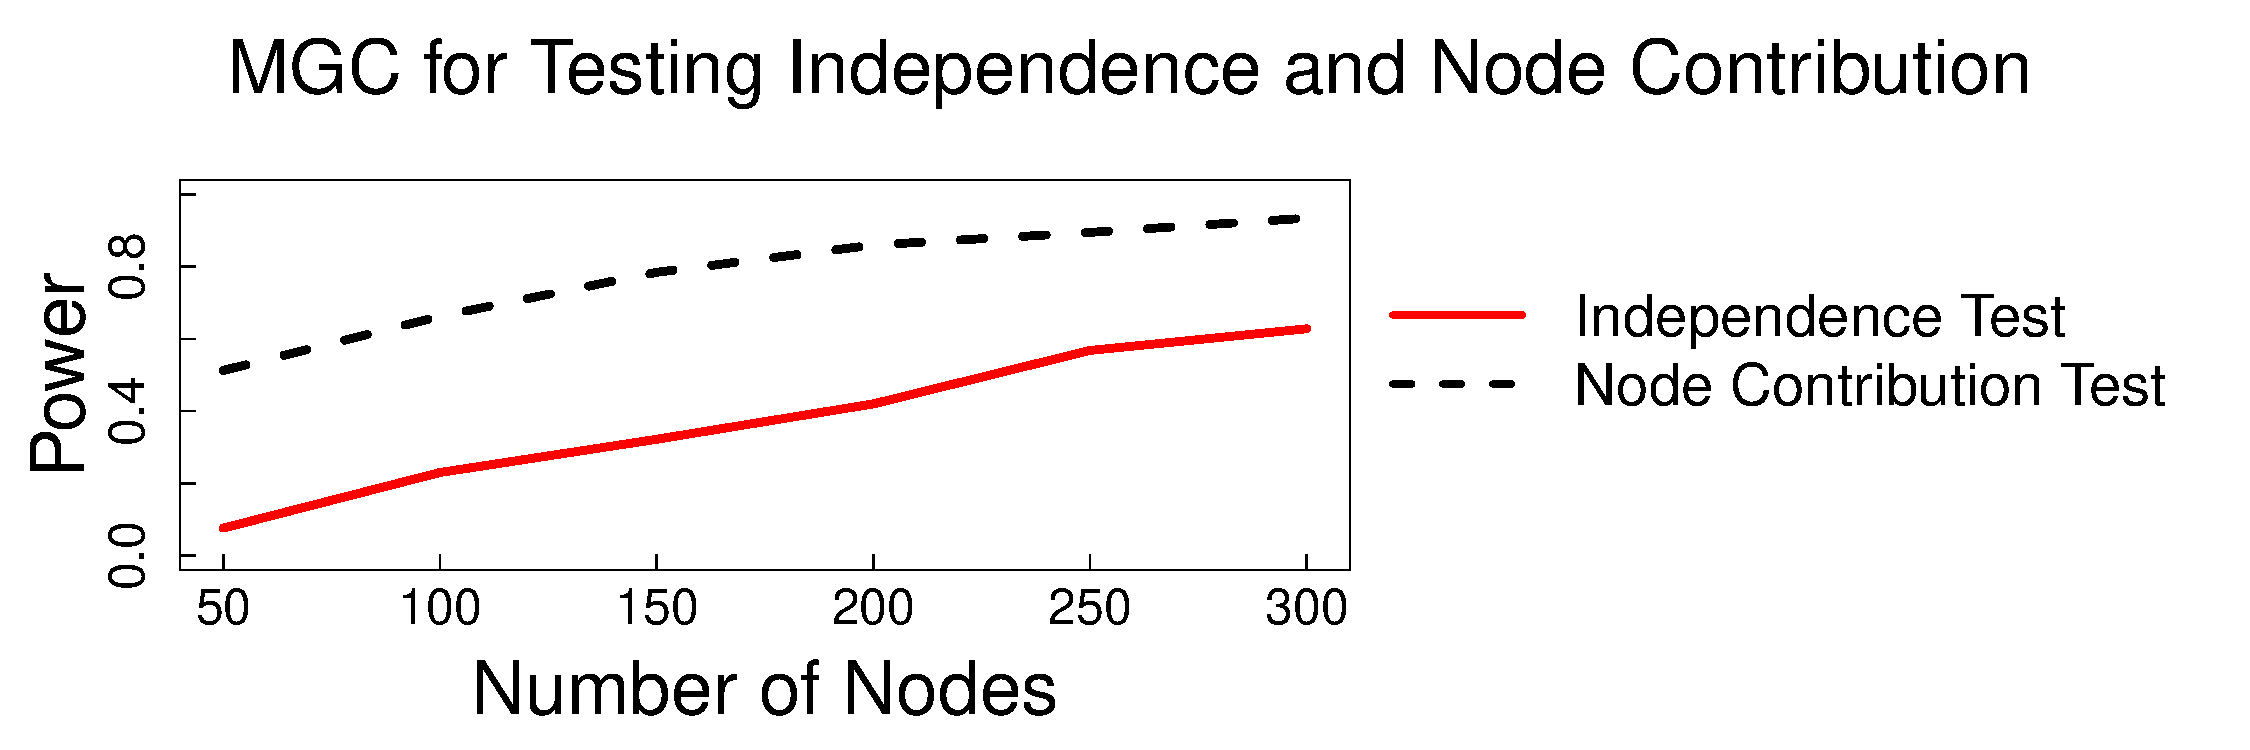
\includegraphics[width=\linewidth]{nodecontri.pdf}
%	\caption{This plot describes that both power of \texttt{MGC} and the rate of correctly-ranked node contribution increase as the number of nodes increases when only half of the nodes for each simulation actually are set to be dependent on network, which validates the use of node contribution measure in independence test.}
%	\label{fig:contribution}
%\end{figure}

\begin{figure}[ht]
	\centering
	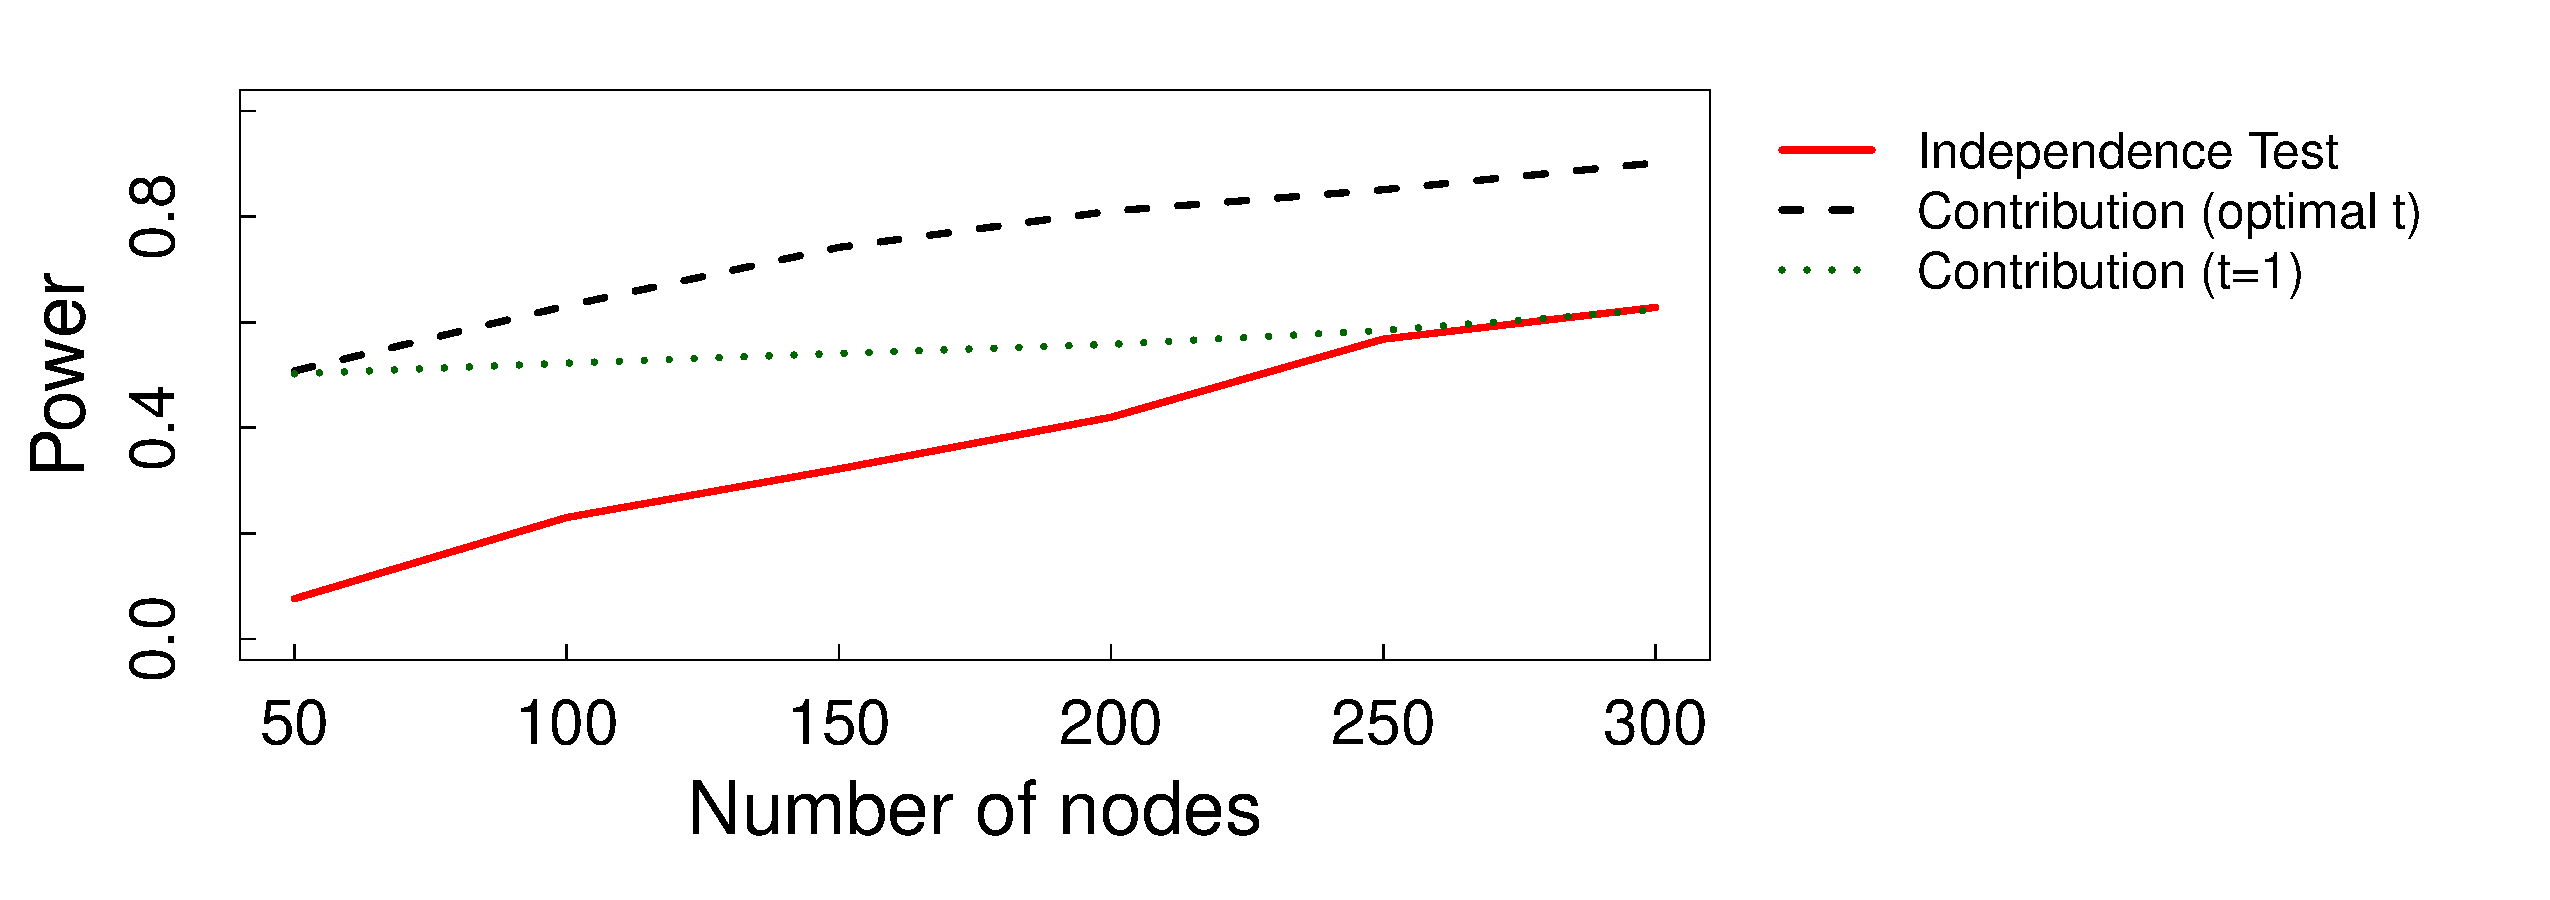
\includegraphics[width=\linewidth]{nodecontri2.pdf}
	\caption{This plot describes that both power of \texttt{MGC} and the rate of correctly-ranked node contribution increase as the number of nodes increases when only half of the nodes for each simulation actually are set to be dependent on network, which validates the use of node contribution measure in independence test.}
	\label{fig:contribution}
\end{figure}
To examine the effectiveness of node contribution measure in testing dependency as presented in the statistic~\ref{eq:contribution}, we deliberately simulate the network and its nodal attributes as half of the nodes are independent while the other half are dependent on network. As an ad hoc test of node contribution, we rank the nodes in terms of decreasing order of $h(v)$ and count the ratio of dependent samples's ranks within the number of dependent nodes. If it works perfectly, all dependent nodes would take higher rank than every independent node so thus the rate equals to one. We call this rate as \textit{inclusion rate}:
\begin{equation}
\mbox{ inclustion rate}\big(  h(v) \big) = \sum\limits_{v \in V(\mathbf{G})} \big\{  rank_{c(v)}\big(  v \big)  \leq  m  \big\}   /  m,
\label{eq:inclusion_rate}
\end{equation}
where $m (\leq |V(\mathbf{G})|)$ is the number of nodes under network dependence. We set $m=n/2$ out of $n = |V(\mathbf{G})|$.


%%%%%%%%%%%%%%%%%%%%%%%%%%%%%%%%%%%%%%%%%
\section{Real Data Examples}
\label{sec:real}
\begin{figure}[ht]
	\centering
	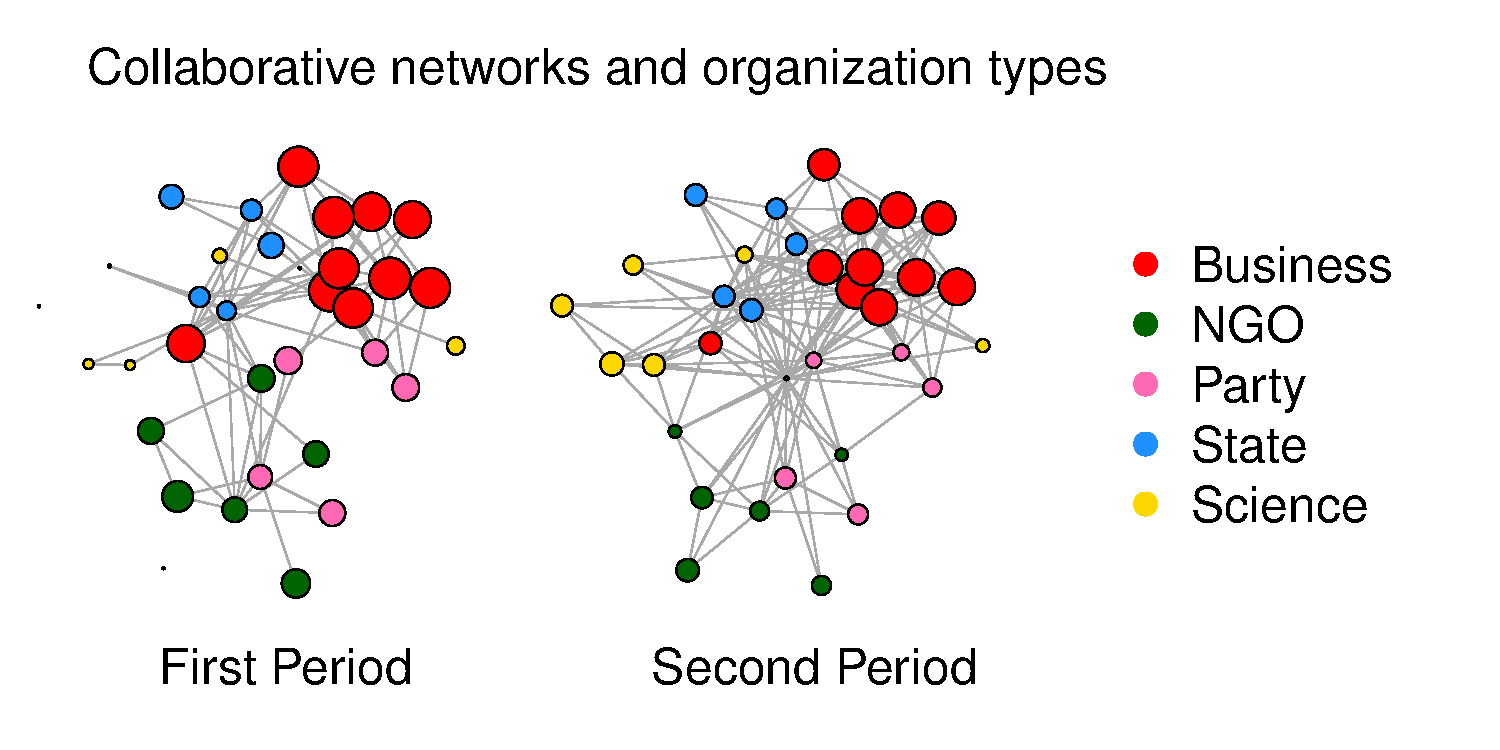
\includegraphics[width=\linewidth]{two_politics.pdf}
	\caption{Both panels depict the collaborative networks during the two time periods having significant network dependency in types of organizations. Using \texttt{MGC} statistics, we are not only able to test network independence but also calculate each node's amount of contribution to detecting dependence, which is proportional to node size here. You can tell that the tendency to collaborate within the same type is strongest among the business group while scientist relatively collaborates less with any others, especially in the first period.}
	\label{fig:politics}
\end{figure}
In the field of political science, who exerts more powerful impacts than the others over political network and which factors impact on the power differentials are one of the interests~\cite{ingold2014structural}. \cite{minhas2016inferential} made an inference from political networks~\cite{cranmer2016navigating} via the additive and multiplicative effects (AME). The AME model estimates the latent factors and uses them to test independence with the nodal attributes. Among diverse attributes that \cite{cranmer2016navigating} provided, we focus on the types of organizations and how 34 political organizations having different types are participating policy network. We changed a given directed network into undirected network and use a dissimilarity matrix for distance matrix of the attributes, i.e., $\parallel \mathbf{X}_{i}  - \mathbf{X}_{j} \parallel = 0$ if and only if node $i$ and node $j$ are from the same type and one otherwise. Two collaboration networks comprised of the same set of nodes across two time periods are provided~\cite{ingold2014structural}. Figure~\ref{fig:politics} and Figure~\ref{fig:barplots} illustrates these two networks and shows each node's reliance on its organization type when collaborating. During the two periods, the network independence test statistics of \texttt{MGC} (p-value : (0.002 , 0.002)) and \texttt{mCorr} (p-value : ( 0.000, 0.000)) using diffusion distance matrices result in significant p-values across diffusion times from $t=1$ to $t=10$. The conclusion from the \texttt{FH} test (p-value : ( 0.000, 0.000)) is also the same.  
\begin{figure}[ht]
	\centering
	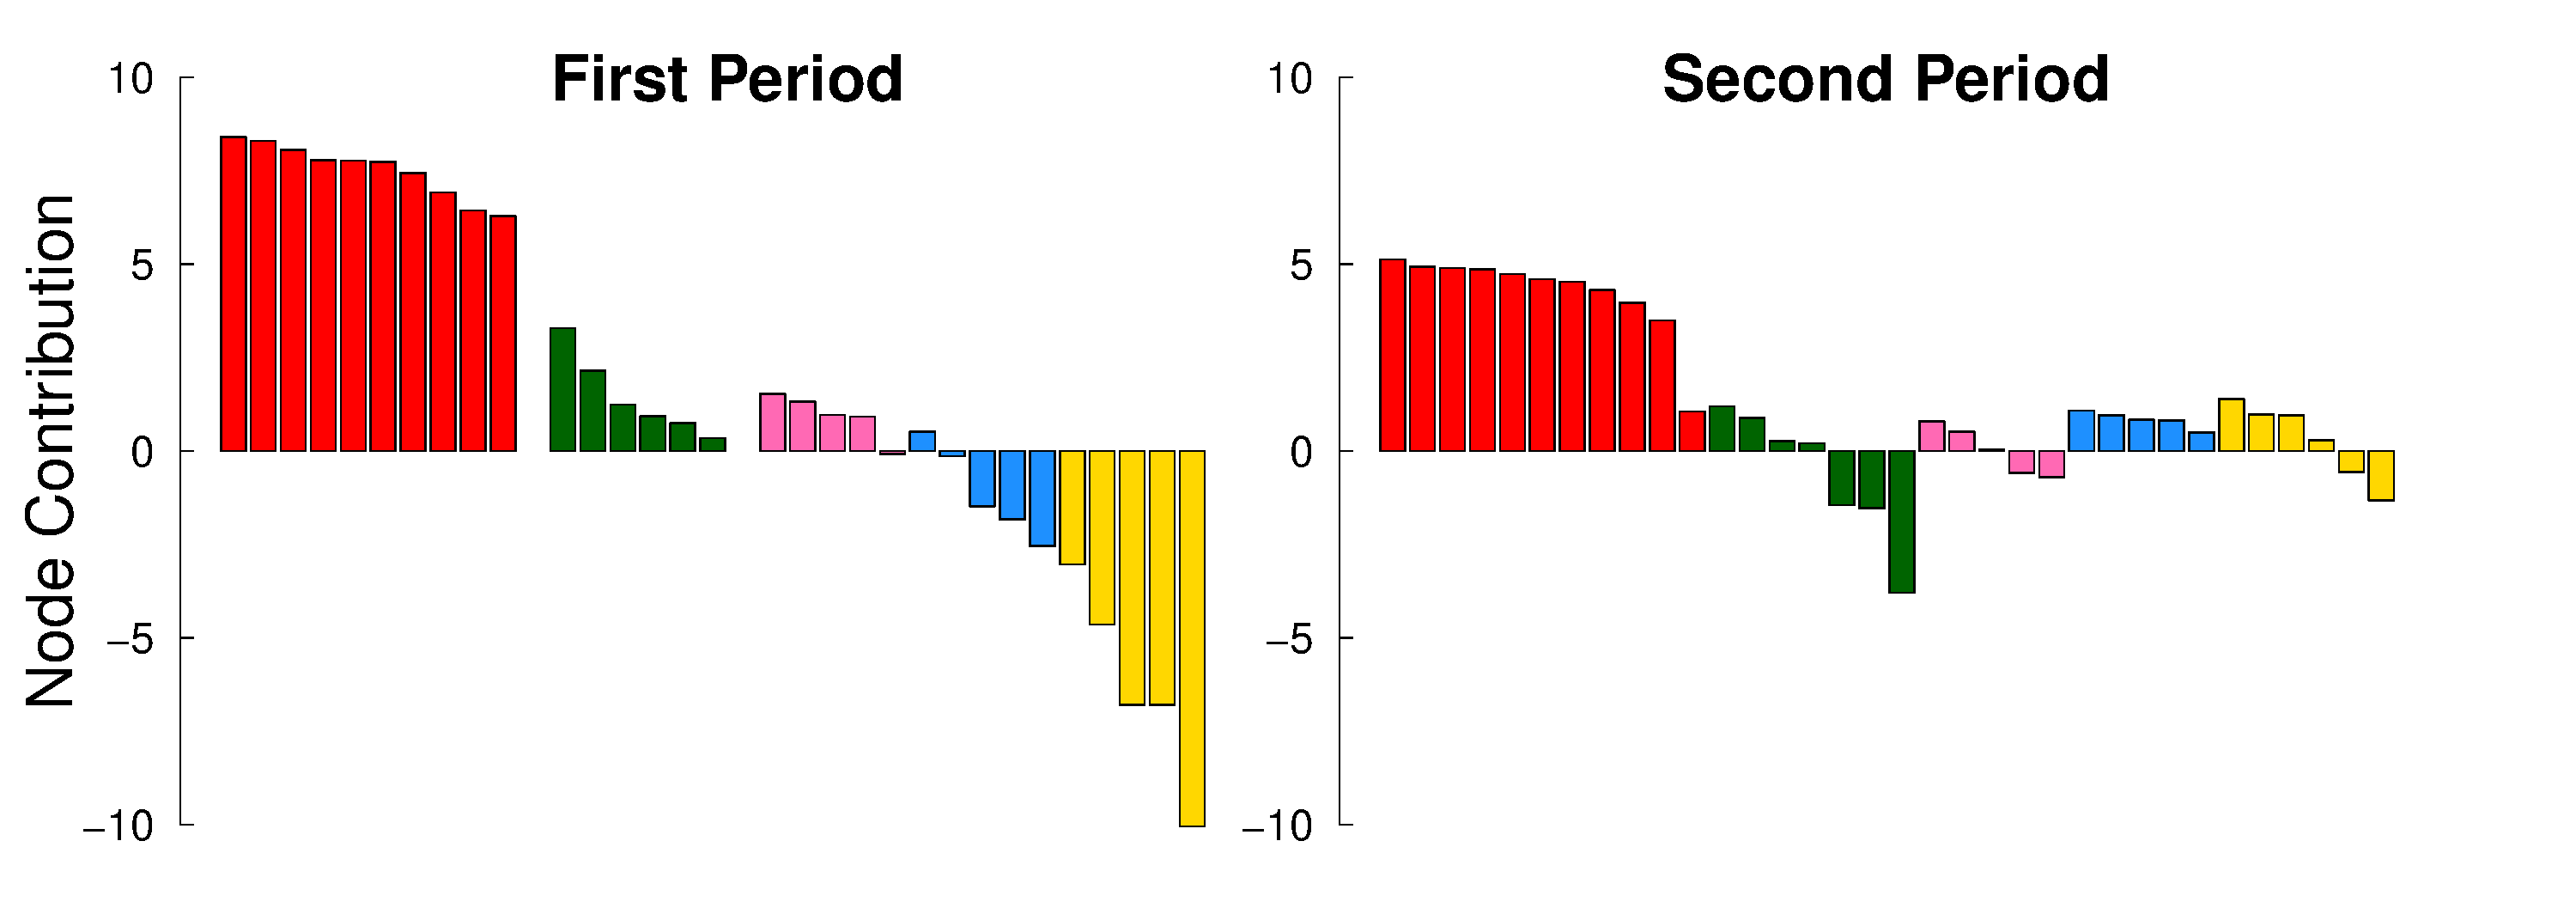
\includegraphics[width=\linewidth]{barplots_nolegend.pdf}	
	\caption{In the first period, we have two extreme cases among the business group and science group, which reflects our observations in Figure~\ref{fig:politics}. Generally organizations cooperate more actively between different types in the second period but still their collaboration network is highly dependent on their organization types especially for business group.}
	\label{fig:barplots}
\end{figure}
\cs{can we expand the real data section? It looks too short for now, although it is probably ok for stat journal.}
\textcolor{red}{I am considering manipulation MRI data in order to show the case where MGC > others... }

%%%%%%%%%%%%%%%%%%%%%%%%%%%%%%%%%%%%%%%%
\vspace*{-0.5cm}
\section{Conclusion And Future Work}
\label{sec:conc}
	\vspace*{-0.2cm}
In this study, we combined recent progress in dependency testing and metric learning into the graph domain, and showed that \texttt{MGC} on the diffusion distance offers an elegant and powerful solution to the network dependency problem, which overcomes many challenges and restraints in the domain of network analysis. We proved that our method is consistent under a mild condition inclusive of almost all popular graph models; and empirically demonstrated it has superior power over all benchmarks, with \texttt{MGC} and the diffusion distance being the core elements behind the success. Moreover we suggested the measure to (relatively) quantify the amount of dependency that each node exhibits. This measure would be very useful when we are not only interested in detecting the network dependence but also in investigating relatively how much is attributable to each node in rejecting network independence.  

There are a number of additional potential extensions of this work. First, how to choose a better diffusion time $t$, or find a $t$ with provable finite-sample performance, may establish more solid foundation of this approach. Second, the network dependence testing here is actually equivalent to the two-sample test, i.e., whether two graphs come from the same distribution; thus our approach readily offers a new nonparametric two-sample test on networks, for which more investigation will bring a valuable addition to the graph analysis. Third, with a few alterations, the new correlation measure on graph may be utilized for other tasks, such as feature screening, outlier detections, clustering, and classification, etc. Fourth, as a next step of this paper, we will utilize this method to a wide range of graphs available in social network and brain analysis, to answer domain specific practical questions.

%convince that \texttt{MGC}, merged with a family of diffusion distance, provides us powerful independence test statistics in network. Having multiscale statistics, i.e.~one parameter family of statistics, is not avoidable because we regard distance between the nodes over network as a dynamic process. Through simulation studies, we demonstrate that our methods perform better than the others especially under nonlinear dependency, and we are able to measure each node's contribution to detecting dependency. Deriving the contributions is particularly important when there have possibly different amounts of the dependencies among the nodes.  

%However obtaining a full family of statistics are computationally infeasible. Also we did not suggest any theoretically supported tools to select one metrics among them so thus we have one single statistic. As an ad hoc, we selected an \textit{optimal} diffusion time $t$ with highest power from $t=1$ to $t=10$ for our simulation since we could observe a stabilized empirical power within this period. Developing the adaptive method to find this optimal $t$ where dependence is maximized would be a natural next step. Despite these shortcomings, we expect that we could also enjoy the properties of \texttt{MGC} and a family of diffusion distances in solving diverse problems which require to utilize local relationship of the data sets. For instance, we might be able to implement independence testing between two networks of same size by using diffusion distance of each network to investigate whether a pair of networks are topologically or structurally independent. This kind of work would shed light on revealing any relationship between the data sets which are not necessarily a random vector.

%%%%%%%%%%%%%%%%%%%%%%%%%%%%%%%%%%%%%%%%%%%%
\newpage
\bibliography{reference}
%%%%%%%%%%%%%%%%%%%%%%%%%%%%%%%%%%%%%%%%%%%%%%
\newpage
\section{Appendix}
\subsection{Proofs}
\label{ssec:proof}

%%%%%%%%%%%%%%%%%%%%%%%%%%%%%%%%%%%%%%%%	
\begin{proof}[\textbf{Proof of Lemma~\ref{main_lemma}}]
To prove conditional \textit{i.i.d.} of the diffusion map $\{\mathbf{u}(i) : i=1,\ldots,n\}$ as $n \rightarrow \infty$, by the celebrated \textit{de Finetti's Theorem}~\cite{diaconis1980finite}, it suffices to prove that $\mathbf{u}(i)$ for $i=1,\ldots,n$ are exchangeable, i.e., for any permutation $\sigma$, the permuted sequence $\mathbf{u}(\sigma(1)), \mathbf{u}(\sigma(2)), \ldots,\mathbf{u}(\sigma(n))$ distributes the same as the original sequence $\mathbf{u}(1), \mathbf{u}(2), \ldots,\mathbf{u}(n)$. Let$\mathbf{V}$ be a $q \times n$ matrix having $\mathbf{u}(i)$ as a $i^{th}$ column $(i = 1, \ldots, n)$. Denoting the permutation matrix as $M$, it is to show that $\mathbf{V}$ always distributes the same as $\mathbf{V} M^{T}$ in matrix notation. 
	
Recall that the diffusion map at time $t$, $\mathbf{u}(i)$ is represented as follows :
\begin{align}
\mathbf{u}(i)  &= \begin{pmatrix} \lambda^{t}_{1} \mathbf{\phi}_{1}(i) & \lambda^{t}_{2} \mathbf{\phi}_{2} (i)  & \cdots & \lambda^{t}_{q} \mathbf{\phi}_{q}(i) \end{pmatrix} \in \mathbb{R}^{q}; \quad i = 1, \ldots, n.
\end{align}

Thus when $\Lambda=diag\{ \lambda_{1},\lambda_2,\ldots,\lambda_q \}$ denotes the diagonal matrix of non-zero eigenvalues and $\Phi =[ \mathbf{\phi}_1, \mathbf{\phi}_2,\cdots, \mathbf{\phi}_q ]$ is the matrix having column vectors as the corresponding eigenvectors of the transition matrix $\mathbf{P}$, $\mathbf{P}=\Phi \Lambda \Phi^{T}$. Then given the graph $\mathbf{G}$ is exchangeable, i.e., $A_{\sigma(i)\sigma(j)} \stackrel{d}{=} A_{ij}$, we have
\begin{align*}
\mathbf{P}_{\sigma(i) \sigma(j)} &= A_{\sigma(i) \sigma(j)} / \sum\limits_{j} A_{\sigma(i)\sigma(j)} \\
 &\stackrel{d}{=} A_{ij} /  \sum\limits_{j} A_{ij} \\
&= \mathbf{P}_{ij},
\end{align*}
 from which it follows that
\begin{align*}
	 M \mathbf{P} M^{T} &\stackrel{d}{=} \mathbf{P} \\
	  \Rightarrow (M \Phi) \Lambda (M \Phi)^{T} &\stackrel{d}{=} \Phi \Lambda \Phi^{T} \\
		\Rightarrow \mathbf{V} M^{T}= \Lambda (M \Phi)^{T} &\stackrel{d}{=} \Lambda \Phi^{T} = \mathbf{V}
\end{align*}	
Therefore, the diffusion maps are exchangeable, and also conditional \textit{i.i.d.} asymptotically by \textit{Finetti’s Theorem}~\cite{diaconis1980finite,orbanz2015bayesian}.
\end{proof}

%%%%%%%%%%%%%%%%%%%%%%%
\begin{proof}[\textbf{Proof of Lemma~\ref{lemma1}} Convergence of empirical characteristic functions of exchangeable variables] 
	This follows exactly the same as \textit{Theorem 1} in \cite{szekely2007measuring}. Note that this Lemma always holds without any assumption on $\{(\mathbf{u}_{i},\mathbf{x}_{j}) :  i=1,2,...,n\}$, e.g., it holds without assuming exchangeability, nor identically distributed, nor finite second moments.
\end{proof}

\begin{proof}[\textbf{Proof of Lemma~\ref{lemma2}} Empirical characteristic function of exchangeable variables] 
	\bigskip	
	It suffices to prove the first argument~\ref{eq:conv1} since the second argument~\ref{eq:conv2} immediately follows from the first one by the property of characteristic functions.
	Proving the first one is equivalent to \textit{Theorem 2} in \cite{szekely2007measuring}. However, they required a given pair of data $\{(\mathbf{u}_{i},\mathbf{x}_{i}) : i = 1, \ldots , n \}$ to be independently identically distributed as $(\mathbf{u},\mathbf{x})$ with finite second moments; here we have exchangeable data $\{  \mathbf{u}_{i} : i = 1, \ldots, n  \}$ instead. 
	
	Followed by \textit{de Finetti's Theorem}~\cite{diaconis1980finite}, if and only if $\{ \mathbf{u}_{i} : i = 1, \ldots, n \}$ are (infinitely) exchangeable, there exists an underlying distribution $f_{\mathbf{u}}$ of $\mathbf{u}$ such that $\mathbf{u}_{i}  \overset{i.i.d}{\sim} f_{\mathbf{u}} $. Then we can also have joint distribution of the data set. Let $(\mathbf{u}_{i}, \mathbf{x}_{i}) \overset{i.i.d}{\sim}   f_{\mathbf{u}, \mathbf{x}}$. Then under the assumption of finite second moment of the underlying distributions and measurable, conditioned random functions, we have a strong large number for V-statistics followed by \cite{szekely2007measuring}, i.e., 
	\begin{eqnarray}
	\displaystyle\int_{D(\delta)}{\|g_{\mathbf{u},\mathbf{x}}^{n}(t,s)-g_{\mathbf{u}}^{n}(t)g_{\mathbf{x}}^{n}(s)\|^{2}}dh &\stackrel{n \rightarrow \infty}{\longrightarrow} 
	\displaystyle\int_{D(\delta)}{\|g_{\mathbf{u},\mathbf{x}}(t,s)-g_{\mathbf{u}}(t)g_{\mathbf{x}}(s)\|^{2}}dh,
	\label{eq:SLLN}
	\end{eqnarray}
	where $D(\delta)=\{(t,s):\delta \leq |t|_{p} \leq 1/\delta,\delta \leq |s|_{q} \leq 1/\delta\}$, and $h(t,s)$ is the weight function chosen in \cite{szekely2007measuring}. 
\end{proof}


%%%%%%%%%%%%%%%%%%%%%%%%
\begin{proof}[\textbf{Proof of Theorem~\ref{theoremMain}} \texttt{MGC} Consistency via Diffusion Distance]

Combining equation~\ref{eq:conv1} and equation~\ref{eq:SLLN} yields
\begin{eqnarray}
\mbox{\texttt{dCov}}(\mathbf{U},\mathbf{X}) &\longrightarrow \displaystyle\int{\|g_{\mathbf{u},\mathbf{x}}(t,s)-g_{\mathbf{u}}(t)g_{\mathbf{x}}(s)\|^{2}}dw,
\label{eq:main2}
\end{eqnarray}
which clearly equals $0$ if and only if independence holds. As distance correlation is just a normalized version of distance covariance, we also have 
\begin{eqnarray}
\mbox{\texttt{dCorr}}(\mathbf{U},\mathbf{X}) &\longrightarrow 0,
\label{eq:main1}
\end{eqnarray}
if and only if the diffusion maps $\mathbf{U}$ is independent of the nodal attributes $\mathbf{X}$.

By \cite{shen2016discovering}, Equation~\ref{eq:main1} holds under the same condition, when \texttt{dCorr} is replaced by \texttt{MGC}. Therefore, both \texttt{MGC} and \texttt{dCorr} are consistent in network dependence testing between the diffusion maps $\mathbf{U}$ and the nodal attributes $\mathbf{X}$.
\end{proof}

%%%%%%%%%%%%%%%%%%%%%%%%%%%%%%%%%%%%%%%%
\subsection{Diffusion Distance in Directed Graphs}
\label{ssec:directed}

However, when a graph is directed, a kernel of an adjacency matrix is not symmetric. Thus, keeping the formal definition of diffusion distance~\ref{eq:distance}, we have a slightly different representation from Equation~\ref{eq:diffusion} main due to $\pi(i) P_{ij} \neq \pi(j) P_{ji}$. Let $\tilde{\mathbf{P}}$ be a time-reversal or transpose matrix of $\mathbf{P}$.

\begin{equation}
\begin{split}
\label{eq:directed}
C^2_{t}(i,j)  & = \big( \mathbf{P}^{t} \tilde{ \mathbf{P} }^{t} \Pi^{-1} \big)(i,i) - \big( \mathbf{P}^{t} \tilde{ \mathbf{P} }^{t} \Pi^{-1} \big)(j,i) \\ & = \big( \mathbf{P}^{t} \tilde{ \mathbf{P} }^{t} \Pi^{-1} \big)(j,j) - \big( \mathbf{P}^{t} \tilde{ \mathbf{P}}^{t} \Pi^{-1} \big) (i,j),
\end{split}  
\end{equation}
where a $\Pi$ is a diagonal matrix with diagonal terms of $\{ \pi(u) : u \in V \}$. 
Different from the former undirected case, $\Pi^{1/2} \mathbf{P} \Pi^{-1/2}$ does not yield a symmetric matrix which results in a concise representation of $\mathbf{P}$. Tang~\cite{tang2010graph} claims that embedding of $C_{t}$ using the eigenvalues and eigenvectors of $\mathbf{P}$ is not possible, even though it is shown that the diffusion distance in directed graph is still Type-2 Euclidean distance matrix (EDM-2) when $\mathbf{P}$ is irreducible. 
%%%%%%%%%%%%%%%%%%%%%%%%%%%%%%%%%%%%%%%%%%%%%
\subsection{Algorithms}
\alglanguage{pseudocode}

\begin{algorithm}[ht]
	\caption{Mutiscale representation of nodes in network}
	\begin{algorithmic}[1]
		\Require Transition probability matrix $P$ of network $G$ and a set of time points $\{ t_{i}  : t_{i} \in \mathbb{N} \}$  of diffusion time. 
		\Ensure A list of diffusion maps at each time point.
		\Function{ \texttt{dmap} }{ $n \times n$ transition matrix $P$, time points $\{ t_{1}, t_{2}, \ldots, t_{K} \}$ } 
		\State $\mathbf{\pi} :=$ \texttt{statdistr}($P$)\Comment{stationary distribution of $P$} 
		\State $\Pi : =$ \texttt{Diag}($\mathbf{\pi}$)\Comment{Diagonal matrix with diagonal element of $\mathbf{\pi}$}
		\State $Q: = \Pi^{1/2} P \Pi^{-1/2}$ 
		\State $\lambda := $ \texttt{eigenvalue}($Q$)\Comment{a real-valued vector with length of $q (\leq n)$. }
		\State $\Lambda : =$ \texttt{Diag}($\lambda$)
		\State $\Psi : =$ \texttt{eigenfunction}($Q$)\Comment{$n \times q$ real-valued matrix} 
		\State $\Phi :=  \Pi^{-1/2} \Psi$\Comment{$n \times q$ real-valued eigenfunction matrix of $P$}
		\For{$t_{i}$ :  $i$ = 1 }{ $K$}
		\Begin
		\State \texttt{Maps}$[i] := \Phi \Lambda^{t_{i}}$  
		\End
		\EndFor
		\State \texttt{Maps} = list( \texttt{Maps}[1], \texttt{Maps}[2], $\ldots$, \texttt{Maps}[$K$]  )
		
		\Return \texttt{Maps}
		\EndFunction
	\end{algorithmic}
\end{algorithm}

%%%%%%%%%%%%%%%%%%%%%%%%%%%%%%%%%%%%%%%%%%%%%%%%%%
\begin{algorithm}[ht]
	\caption{Multiscale Generalized Correlation (\texttt{MGC}) test statistics with diffusion maps as a network-based distance.}
	\begin{algorithmic}[1]
		\Require A connected, undirected network $G$ with its nodal attributes $\mathbf{X}$.
		\Ensure A list of \big(  (a) p-value of \texttt{sample MGC}, (b) estimated \texttt{sample MGC} statistic, (c) p-value map for all local correlations, (d) a set of estimated optimal neighborhood scales $\{  (k^{*}, l^{*}  ) \}$  \big) for each diffusion maps.
		\Function{ \texttt{NetworkTest} }{ $G$, $\textbf{X}$,  $\mathbf{T}$ := (diffusion time points $\{ t_{1}, t_{2}, \ldots, t_{K} \}$)  }
		\State $A :=$ \texttt{get.adjacency}$(G)$\Comment{obtain an adjacency matrix of network $G$}
		\State $P := A $ / \texttt{rowSums}($A$) 
		\State $U :=$ \texttt{dmap}($P$, $\mathbf{T}$) \Comment{a list of diffusion maps in each time point}
		\For{$t_{i}$ :  $i$ = 1 }{ $K$}
		\Begin
		\State $C : =$  \texttt{dist}($U[i]$) \Comment{distance matrix of diffusion maps at time $t_{i}$}
		\State $D : =$ \texttt{dist}($X$) \Comment{distance matrix of nodal attributes}
		\State \texttt{MGC}$[i]$ = \texttt{MGCPermutationTest}( $C$, $D$ ) 
		\End
		\EndFor
		\State \texttt{MGC} = list( \texttt{MGC}[1], \texttt{MGC}[2], $\ldots$, \texttt{MGC}[$K$]  )
		
		\Return \texttt{MGC}
		\EndFunction
	\end{algorithmic}
\end{algorithm}

%%%%%%%%%%%%%%%%%%%%%%
\begin{algorithm}[ht]
	\caption{Node-specific contribution to detecting dependency via \texttt{MGC} statistic}
	\begin{algorithmic}[1]
		\Require Distance metric of graph $G$, $C$, and attributes $X$, $D$, and (one of) the estimated optimal scales $\{ k^{*}, l^{*} \}$ 
		\Ensure  unstandardized contributions of each node in network $\{  c(v) \}$
		\Function{ \texttt{Contribution} }{   C, D , $\{  (k^{*}, l^{*}) \}$   }
		\State $\tilde{C} : = \texttt{DoubleCentering}(C)$
		\State $\tilde{D} := \texttt{DoubleCentering}(D)$
		\State \texttt{Rank}($M_{ij}$):= (rank of node $j$ with respect to node $i$)
		\For{$v = 1$}{ $|V(G)|$} \Comment{iterate over every each node}
		\State $c(v) = 0$
		\For{$j = 1$}{ $n$}
		\Begin
		\State $c(v) =  c(v) + \tilde{C}_{vj} \tilde{D}_{v j} I(  \texttt{Rank}(C_{vj})  \leq k^{*}, \texttt{Rank}(D_{vj}) \leq l^{*} )$
		\End
		\EndFor
		\EndFor
		\State \texttt{cset} $:= \{ c(v) : v = 1,2, \ldots , |V(G)|  \}$	
		
		\Return  \texttt{cset}
		\EndFunction
	\end{algorithmic}
\end{algorithm}
%%%%%%%%%%%%%%%%%%%%%%%%%%%%%%%%%%%%%%%%%%%%%%%%%%%
\bigskip
\begin{center}
	{\large\bf SUPPLEMENTARY MATERIAL}
\end{center}

All of the \texttt{R} functions and simulation data in \texttt{RData} format are provided in \url{https://github.com/neurodata/Multiscale-Network-Test}.

%%%%%%%%%%%%%%%%%%%%%%%%%%5
%\begin{proof}[\textbf{Proof of Theorem~\ref{theorem2}} Consistency of \texttt{MGC} applied to exchangeable variables]
	
%Under the exchangeability and finite second moment assumptions of underlying distribution, $\mathcal{V}^{2}_{n}(\mathbf{W},\mathbf{Y}) \xrightarrow{n \rightarrow \infty}  0$ if and only if underlying distribution of $\{\mathbf{w}_{i} \}$, $f_{\mathbf{w}}$ is independent from underlying distribution of $\{ \mathbf{y}_{i}  \}$, $f_{\mathbf{y}}$. Now suppose that we have undirected, connected network $\mathbf{G}$ with a family of diffusion maps $\{ \mathbf{u}_{t}  \}$ and with nodal attributes $\{ \mathbf{x}  \}$. We have shown in the Lemma~\ref{main_lemma} that $\{ \mathbf{u}_{t}  \}$ are exchangeable for each $t \in \mathbb{N}$. Thus there exists an underlying distribution of $\mathbf{u}_{t}$ such that $\mathbf{u}_{t}(i) \overset{i.i.d}{\sim} f_{\mathbf{u}^{(t)}}$ for each of $t= 1,2,\ldots $; and we have $\mathbf{x}_{i} \overset{i.i.d}{\sim} f_{\mathbf{X}}$. Under the assumption of finite second moment of $\mathbf{u}^{(t)}$ and $\mathbf{x}$, \texttt{MGC} statistics constructed by $\{  (  \mathbf{u}_{t}(i), \mathbf{x}_{i} ) : i = 1,2,\ldots, n  \}$ yield a consistent testing which determines the independence between underlying distributions of $\mathbf{u}^{(t)}$ and $\mathbf{x}$. From the same setting of network $\mathbf{G}$, we have estimated \textit{i.i.d} node-specific network factors $\{ \mathbf{F}_{i} \}$ so that $n$-pair of \textit{i.i.d} $\{ ( \mathbf{F}_{i}, \mathbf{x}_{i} )  \}$ can be applied to \texttt{MGC} or other distance-based tests without assuming conditioning underlying distribution. In case of using adjacency matrix directly into test, we must assume that the adjacency matrix comes from connected directed network, i.e. $A_{ij} \overset{i.i.d}{\sim} f_{A}$ for all $i,j=1,2,\ldots, n$; otherwise, each column is dependent on one another.  
%\end{proof}

\end{document}